\documentclass[11pt]{article}
\usepackage[T1]{fontenc}
\usepackage[polish]{babel}
\usepackage{amsmath}
%\usepackage{amssymb}
%\topmargin -2cm
%\textheight 23cm
%\oddsidemargin -1cm
%\evensidemargin -1cm
%\textwidth 17.5cm
\usepackage[lmargin=1cm,rmargin=1.5cm,tmargin=1cm,bmargin=2cm]{geometry}
\usepackage{natbib}
\usepackage{graphicx}
\usepackage{tikz}
\usepackage{pgfplots}
% \usepgfplotslibrary{external} 
% \tikzexternalize[prefix=figures/]
\usetikzlibrary{intersections}
\usetikzlibrary{backgrounds}
\usepackage{minted}
\usepackage{listings}

\usepackage[mathletters]{ucs}
\usepackage[utf8x]{inputenc}

\pgfplotsset{compat=newest}

\title{Model Isinga 2D}
\author{Michał Łukomski}
\date{Styczeń 2021}

\begin{document}

\maketitle

 Symulacje zostały przeprowadzone na sieciach o rozmiarze $L^2$ dla $L \in \{6,20,70\}$. Temperaturę wyrażono w jednostkach zredukowanych $T^* = \frac{k_B}{J} T$. %(do obliczeń, energię również wyrażono w jednostkach zredukowanych $E^* = E/J$)\\

Symulacje startowano z konfiguracjami losowymi - każdemu węzłowi przypisywano stan +1 lub -1 z równym prawdopodobieństwem 1/2. Sieci zostały poddane ewolucji przez $30 000 MCS$, (1$MCS$ = iteracyjne przejście po wszystkich węzłach układu) a następnie przez kolejne $400 000 MCS$, podczas których magnetyzacja była próbkowana co $100 MCS$. Otrzymano więc próbki o rozmiarach 4000, które wykorzystano do obliczeń średniej magnetyzacji, podatności magnetycznej oraz pojemności cieplnej układu. Wyniki przedstawiono na wykresach.

Zakresy temperatur używane w symulacjach to
\begin{itemize}
    \centering
    \item $[0.5; 1.75]$ ze skokiem $\Delta T^* = 0.05$
    \item $[1.8; 2.7]$  ze skokiem $\Delta T^* = 0.005$
    \item $[2.75; 3.5]$ ze skokiem $\Delta T^* = 0.05$
\end{itemize}


Poniżej przedstawiono zaobserwowane układy dla temperatur $T^* = 0.05, T^* = 2.269 \approx T^*_C, T^* = 8.0$. Kolor niebieski oznacza węzeł w stanie -1, a czerwony w stanie +1.

\begin{figure}
    \centering
    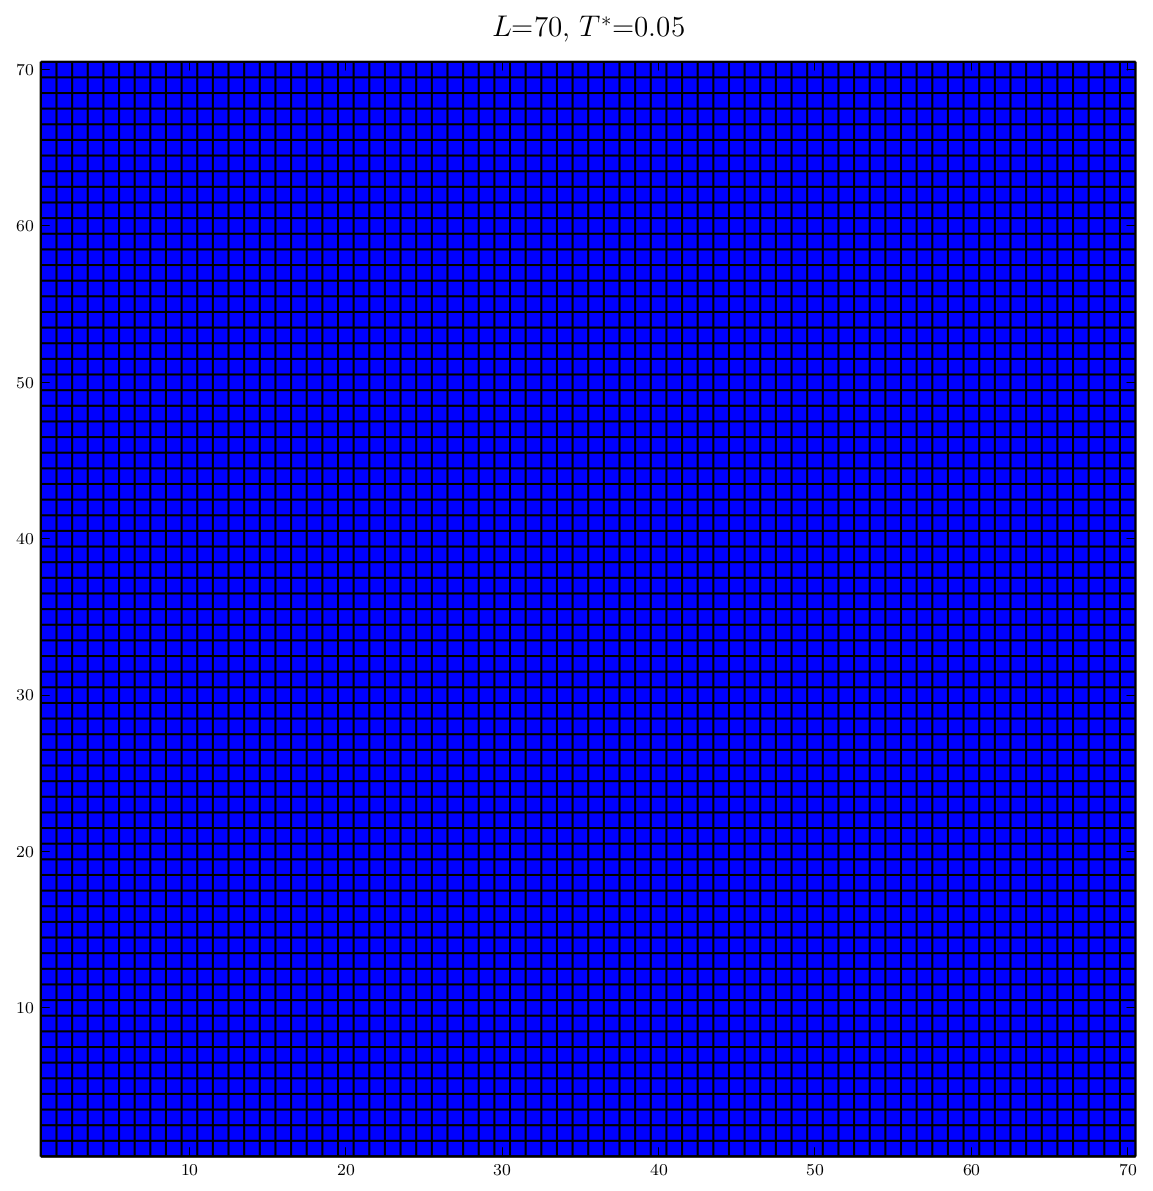
\includegraphics[width=\textwidth]{lattice_L70_T0.png}
    \caption{Konfiguracja dla $L=70$ i $T^* = 0.050$ po $430 000 MCS$. 
    Kolor niebieski to stan -1, a czerwony +1}
\end{figure}
\begin{figure}
    \centering
    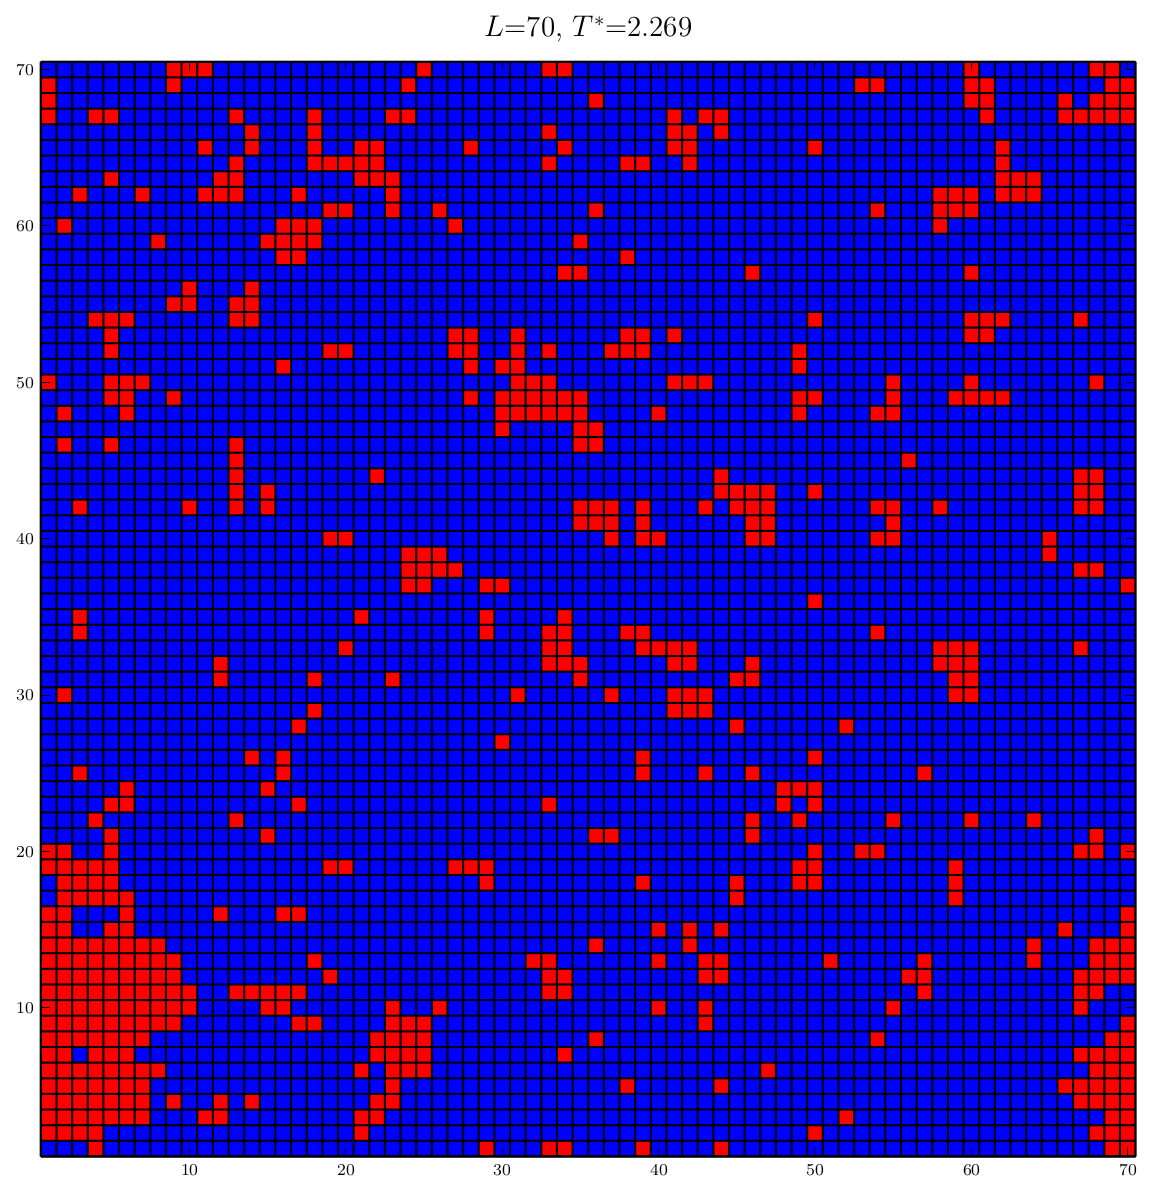
\includegraphics[width=\textwidth]{lattice_L70_T2.png}
    \caption{Konfiguracja dla $L=70$ i $T^* = 2.269$ po $430 000 MCS$. 
    Kolor niebieski to stan -1, a czerwony +1}
\end{figure}
\begin{figure}
    \centering
    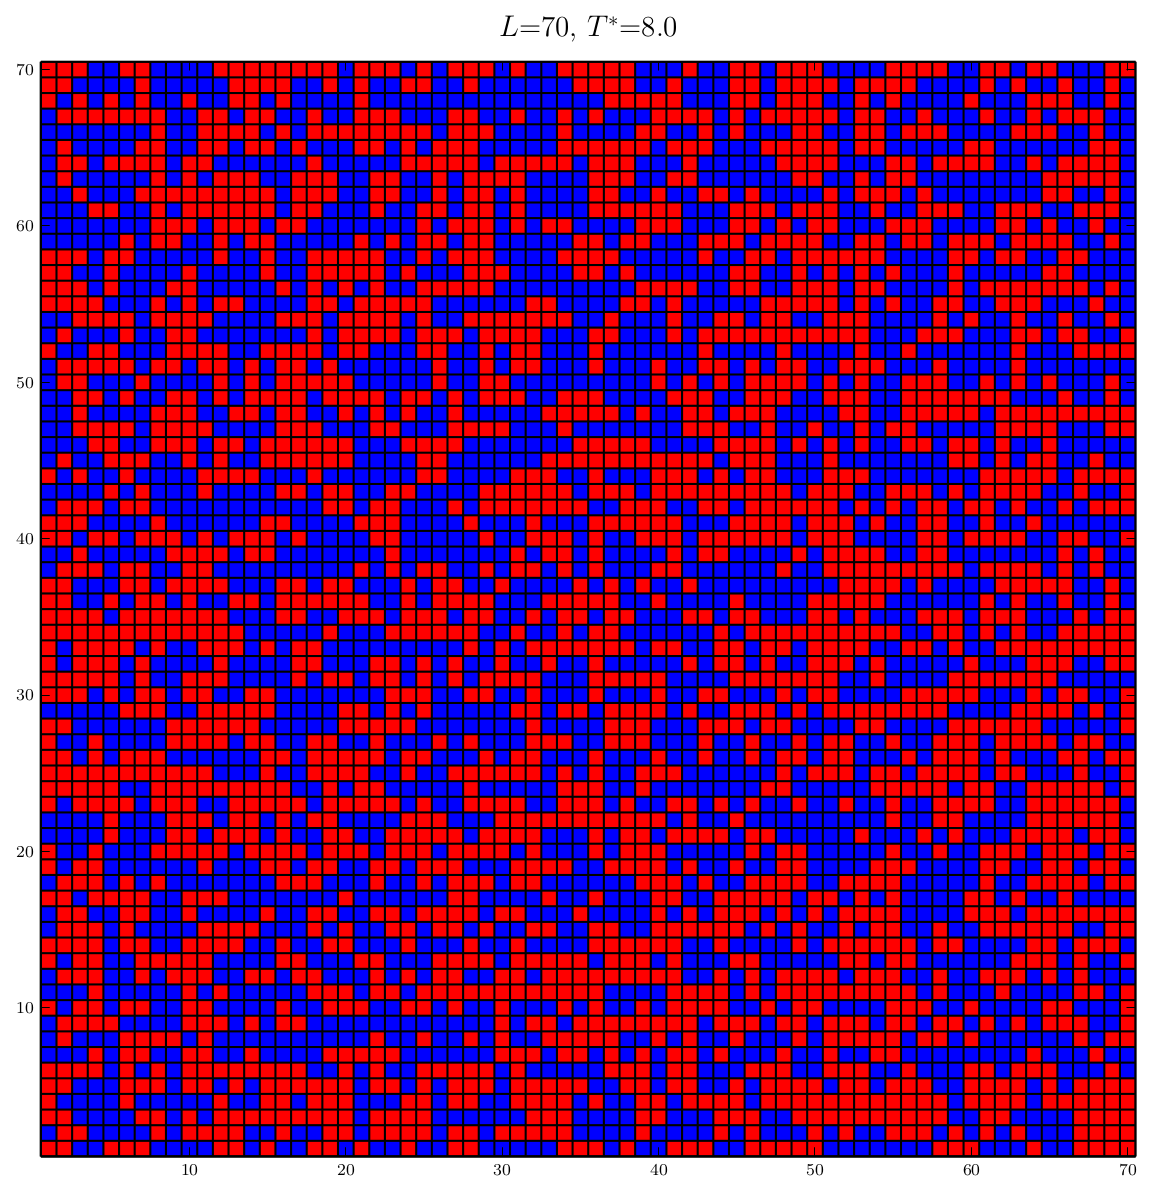
\includegraphics[width=\textwidth]{lattice_L70_T8.png}
    \caption{Konfiguracja dla $L=70$ i $T^* = 8.000$ po $430 000 MCS$. 
    Kolor niebieski to stan -1, a czerwony +1}
\end{figure}
% \begin{figure}
%     \centering
%     \include{lattice_L70_T8}
% \end{figure}
\begin{figure}
    \centering
    \begin{tikzpicture}[/tikz/background rectangle/.style={fill={rgb,1:red,1.0;green,1.0;blue,1.0}, draw opacity={1.0}}, show background rectangle]
\begin{axis}[point meta max={nan}, point meta min={nan}, legend cell align={left}, title={Magnetization as a function of reduced temperature - random initial conditions}, title style={at={{(0.5,1)}}, anchor={south}, font={{\fontsize{10 pt}{13.0 pt}\selectfont}}, color={rgb,1:red,0.0;green,0.0;blue,0.0}, draw opacity={1.0}, rotate={0.0}}, legend style={color={rgb,1:red,0.0;green,0.0;blue,0.0}, draw opacity={1.0}, line width={1}, solid, fill={rgb,1:red,1.0;green,1.0;blue,1.0}, fill opacity={1.0}, text opacity={1.0}, font={{\fontsize{8 pt}{10.4 pt}\selectfont}}, at={(1.02, 1)}, anchor={north west}}, axis background/.style={fill={rgb,1:red,1.0;green,1.0;blue,1.0}, opacity={1.0}}, anchor={north west}, xshift={1.0mm}, yshift={-1.0mm}, width={145.4mm}, height={99.6mm}, scaled x ticks={false}, xlabel={$T^*$}, x tick style={color={rgb,1:red,0.0;green,0.0;blue,0.0}, opacity={1.0}}, x tick label style={color={rgb,1:red,0.0;green,0.0;blue,0.0}, opacity={1.0}, rotate={0}}, xlabel style={at={(ticklabel cs:0.5)}, anchor=near ticklabel, font={{\fontsize{11 pt}{14.3 pt}\selectfont}}, color={rgb,1:red,0.0;green,0.0;blue,0.0}, draw opacity={1.0}, rotate={0.0}}, xmajorgrids={true}, xmin={0.41000000000000003}, xmax={3.59}, xtick={{0.5,1.0,1.5,2.0,2.5,3.0,3.5}}, xticklabels={{$0.5$,$1.0$,$1.5$,$2.0$,$2.5$,$3.0$,$3.5$}}, xtick align={inside}, xticklabel style={font={{\fontsize{8 pt}{10.4 pt}\selectfont}}, color={rgb,1:red,0.0;green,0.0;blue,0.0}, draw opacity={1.0}, rotate={0.0}}, x grid style={color={rgb,1:red,0.0;green,0.0;blue,0.0}, draw opacity={0.1}, line width={0.5}, solid}, axis x line*={left}, x axis line style={color={rgb,1:red,0.0;green,0.0;blue,0.0}, draw opacity={1.0}, line width={1}, solid}, scaled y ticks={false}, ylabel={$<m>$}, y tick style={color={rgb,1:red,0.0;green,0.0;blue,0.0}, opacity={1.0}}, y tick label style={color={rgb,1:red,0.0;green,0.0;blue,0.0}, opacity={1.0}, rotate={0}}, ylabel style={at={(ticklabel cs:0.5)}, anchor=near ticklabel, font={{\fontsize{11 pt}{14.3 pt}\selectfont}}, color={rgb,1:red,0.0;green,0.0;blue,0.0}, draw opacity={1.0}, rotate={0.0}}, ymajorgrids={true}, ymin={-0.0004610714285714253}, ymax={1.0291396428571429}, ytick={{0.0,0.25,0.5,0.75,1.0}}, yticklabels={{$0.00$,$0.25$,$0.50$,$0.75$,$1.00$}}, ytick align={inside}, yticklabel style={font={{\fontsize{8 pt}{10.4 pt}\selectfont}}, color={rgb,1:red,0.0;green,0.0;blue,0.0}, draw opacity={1.0}, rotate={0.0}}, y grid style={color={rgb,1:red,0.0;green,0.0;blue,0.0}, draw opacity={0.1}, line width={0.5}, solid}, axis y line*={left}, y axis line style={color={rgb,1:red,0.0;green,0.0;blue,0.0}, draw opacity={1.0}, line width={1}, solid}]
    \addplot[color={rgb,1:red,0.0;green,0.6056;blue,0.9787}, name path={4599d999-a697-4a22-8293-5926079f8bba}, only marks, draw opacity={1.0}, line width={0}, solid, mark={*}, mark size={2.25 pt}, mark repeat={1}, mark options={color={rgb,1:red,0.0;green,0.0;blue,0.0}, draw opacity={0.1}, fill={rgb,1:red,0.0;green,0.6056;blue,0.9787}, fill opacity={1.0}, line width={0.75}, rotate={0}, solid}]
        table[row sep={\\}]
        {
            \\
            1.2  0.997  \\
            2.37  0.7531805555555554  \\
            2.75  0.5419583333333334  \\
            2.235  0.815597222222222  \\
            1.865  0.9462638888888886  \\
            2.065  0.8899999999999997  \\
            1.35  0.9932777777777776  \\
            2.62  0.6058611111111111  \\
            2.24  0.8200277777777776  \\
            0.95  0.999638888888889  \\
            1.55  0.9839444444444442  \\
            2.445  0.7155833333333332  \\
            2.95  0.4624722222222222  \\
            1.955  0.9238055555555552  \\
            2.025  0.9086944444444441  \\
            2.08  0.8848194444444442  \\
            2.535  0.6548333333333333  \\
            2.135  0.8651944444444442  \\
            2.25  0.8210972222222219  \\
            2.19  0.838958333333333  \\
            1.6  0.9797638888888887  \\
            3.15  0.40301388888888884  \\
            2.04  0.9010416666666663  \\
            1.85  0.9478611111111107  \\
            1.65  0.9743194444444441  \\
            2.34  0.7678749999999999  \\
            2.21  0.8318749999999999  \\
            2.4  0.7397499999999998  \\
            2.22  0.8304722222222221  \\
            2.39  0.7344861111111111  \\
            1.815  0.9526388888888885  \\
            2.02  0.9111805555555552  \\
            1.25  0.9960138888888888  \\
            2.085  0.8887777777777774  \\
            1.95  0.9258749999999997  \\
            0.8  0.9999166666666668  \\
            1.05  0.999  \\
            2.09  0.8858055555555552  \\
            0.5  1.0  \\
            1.845  0.9495694444444441  \\
            0.55  1.0  \\
            2.8  0.52875  \\
            2.605  0.6240416666666667  \\
            3.35  0.3613333333333333  \\
            2.215  0.8300277777777776  \\
            2.205  0.8312916666666664  \\
            2.565  0.6309166666666668  \\
            2.525  0.6636111111111109  \\
            1.895  0.9401666666666664  \\
            2.07  0.8896249999999998  \\
            1.855  0.9466388888888885  \\
            2.415  0.7290972222222222  \\
            2.255  0.8060138888888887  \\
            1.45  0.9890416666666665  \\
            2.595  0.6276666666666667  \\
            2.315  0.7768888888888889  \\
            2.285  0.7961805555555553  \\
            2.58  0.6328055555555556  \\
            2.355  0.7641249999999998  \\
            1.885  0.940583333333333  \\
            2.045  0.9005972222222219  \\
            2.85  0.49993055555555554  \\
            2.555  0.6443888888888889  \\
            3.45  0.34191666666666665  \\
            2.675  0.5810416666666667  \\
            2.27  0.8008611111111109  \\
            2.35  0.7621805555555554  \\
            2.26  0.806722222222222  \\
            2.2  0.8392361111111108  \\
            0.7  0.9999583333333334  \\
            2.385  0.7448611111111111  \\
            1.83  0.951333333333333  \\
            1.805  0.9541944444444441  \\
            2.06  0.8950972222222219  \\
            2.225  0.8339999999999997  \\
            1.89  0.9379444444444441  \\
            2.275  0.802986111111111  \\
            2.52  0.6683055555555557  \\
            2.695  0.5778888888888888  \\
            2.3  0.7900416666666665  \\
            1.945  0.9263055555555552  \\
            2.65  0.5962916666666668  \\
            1.0  0.999375  \\
            1.88  0.9434583333333331  \\
            2.64  0.6026388888888888  \\
            2.13  0.8707777777777775  \\
            2.16  0.8531527777777776  \\
            2.005  0.9094444444444442  \\
            0.9  0.999638888888889  \\
            2.365  0.7535694444444443  \\
            2.475  0.6951388888888888  \\
            1.75  0.9630555555555553  \\
            2.335  0.7719305555555553  \\
            1.835  0.9494027777777774  \\
            1.99  0.9175833333333331  \\
            2.18  0.8497638888888887  \\
            2.45  0.7078749999999999  \\
            2.665  0.5903055555555554  \\
            1.8  0.9559861111111108  \\
            3.2  0.39795833333333336  \\
            2.655  0.5810138888888889  \\
            2.455  0.7018194444444443  \\
            1.92  0.9359444444444441  \\
            2.175  0.8466805555555554  \\
            1.84  0.9481111111111109  \\
            2.125  0.8686805555555552  \\
            2.57  0.6422499999999999  \\
            1.925  0.9305138888888884  \\
            2.42  0.7234305555555555  \\
            2.28  0.7994444444444442  \\
            2.195  0.8439999999999998  \\
            2.54  0.658625  \\
            1.94  0.9293194444444441  \\
            1.86  0.9470972222222219  \\
            1.995  0.912958333333333  \\
            1.935  0.9322916666666663  \\
            0.6  1.0  \\
            2.59  0.6243194444444443  \\
            2.0  0.913458333333333  \\
            1.5  0.9867638888888887  \\
            2.68  0.5844166666666667  \\
            1.4  0.9912916666666665  \\
            2.17  0.853458333333333  \\
            1.975  0.9178749999999997  \\
            2.295  0.793486111111111  \\
            2.575  0.6320694444444444  \\
            2.33  0.7712083333333333  \\
            2.245  0.8225277777777776  \\
            2.66  0.5940972222222223  \\
            2.685  0.5828333333333332  \\
            2.41  0.7275138888888889  \\
            2.11  0.8783055555555555  \\
            2.69  0.5742222222222222  \\
            2.31  0.7884583333333332  \\
            2.47  0.6941944444444443  \\
            1.98  0.9211666666666662  \\
            2.03  0.9073611111111108  \\
            2.425  0.7218888888888888  \\
            2.585  0.6232083333333333  \\
            2.165  0.8541944444444443  \\
            1.1  0.9985694444444445  \\
            1.3  0.9950277777777776  \\
            2.645  0.5927361111111111  \\
            2.49  0.6799166666666667  \\
            2.43  0.7171944444444444  \\
            0.75  0.9999305555555555  \\
            2.38  0.7485416666666665  \\
            2.435  0.7102777777777776  \\
            2.1  0.8832777777777774  \\
            0.85  0.9998055555555556  \\
            2.265  0.8047222222222219  \\
            1.96  0.9239999999999996  \\
            1.985  0.9159027777777775  \\
            2.515  0.664611111111111  \\
            2.485  0.6874999999999999  \\
            2.105  0.8757916666666665  \\
            2.055  0.8953749999999997  \\
            2.01  0.9120972222222218  \\
            1.905  0.9360416666666663  \\
            0.65  1.0  \\
            2.6  0.6214444444444445  \\
            2.305  0.7922916666666665  \\
            2.7  0.5732222222222223  \\
            2.635  0.6054722222222223  \\
            2.29  0.7972777777777776  \\
            1.825  0.9537222222222219  \\
            1.81  0.9559305555555552  \\
            2.395  0.7462638888888887  \\
            2.46  0.7000277777777778  \\
            2.63  0.6065694444444445  \\
            3.3  0.3700555555555555  \\
            1.7  0.9712361111111109  \\
            2.44  0.7127916666666665  \\
            2.405  0.733486111111111  \\
            2.56  0.6520277777777778  \\
            2.075  0.8917361111111108  \\
            2.23  0.8242499999999998  \\
            3.25  0.3848611111111111  \\
            2.015  0.9092638888888884  \\
            2.035  0.9014861111111109  \\
            2.36  0.7564444444444444  \\
            1.82  0.954222222222222  \\
            2.465  0.6977222222222221  \\
            3.5  0.33501388888888883  \\
            2.53  0.6580277777777779  \\
            2.375  0.7453749999999998  \\
            2.325  0.7745555555555553  \\
            1.87  0.9426944444444442  \\
            1.875  0.9457361111111108  \\
            2.51  0.673361111111111  \\
            2.145  0.8601666666666663  \\
            2.15  0.860861111111111  \\
            2.115  0.8756111111111109  \\
            2.48  0.6907222222222221  \\
            2.9  0.47866666666666674  \\
            2.345  0.7663472222222222  \\
            1.9  0.9374722222222219  \\
            1.91  0.9339999999999996  \\
            3.4  0.364875  \\
            2.55  0.6561388888888888  \\
            2.14  0.8626805555555553  \\
            2.095  0.8793749999999997  \\
            2.67  0.5863194444444445  \\
            2.155  0.8571249999999998  \\
            3.0  0.45123611111111106  \\
            1.93  0.9326666666666663  \\
            1.965  0.9234027777777774  \\
            2.5  0.6803749999999998  \\
            1.15  0.9975833333333333  \\
            2.505  0.6782083333333333  \\
            1.915  0.935583333333333  \\
            2.12  0.873847222222222  \\
            2.615  0.6100277777777778  \\
            2.185  0.8484166666666664  \\
            2.495  0.6826111111111111  \\
            3.05  0.43675  \\
            2.32  0.7827499999999997  \\
            2.545  0.6478472222222221  \\
            2.61  0.6214166666666666  \\
            2.05  0.898333333333333  \\
            1.97  0.9209166666666664  \\
            3.1  0.4292361111111111  \\
            2.625  0.609375  \\
        }
        ;
    \addlegendentry {L=6}
    \addplot[color={rgb,1:red,0.8889;green,0.4356;blue,0.2781}, name path={71ee0805-2ff8-41d5-826c-81e023617151}, only marks, draw opacity={1.0}, line width={0}, solid, mark={square*}, mark size={2.25 pt}, mark repeat={1}, mark options={color={rgb,1:red,0.0;green,0.0;blue,0.0}, draw opacity={0.1}, fill={rgb,1:red,0.8889;green,0.4356;blue,0.2781}, fill opacity={1.0}, line width={0.75}, rotate={0}, solid}]
        table[row sep={\\}]
        {
            \\
            1.2  0.9971024999999998  \\
            2.37  0.505125  \\
            2.75  0.17791  \\
            2.235  0.7468212500000001  \\
            1.865  0.9456800000000002  \\
            2.065  0.8861775000000001  \\
            1.35  0.9931074999999997  \\
            2.62  0.23880749999999998  \\
            2.24  0.7398250000000001  \\
            0.95  0.99952875  \\
            1.55  0.9834462499999999  \\
            2.445  0.38208  \\
            2.95  0.14222125  \\
            1.955  0.92444625  \\
            2.025  0.90342375  \\
            2.08  0.8792437500000001  \\
            2.535  0.28957874999999994  \\
            2.135  0.84899  \\
            2.25  0.72570875  \\
            2.19  0.803895  \\
            1.6  0.9795274999999999  \\
            3.15  0.12122625  \\
            2.04  0.89690875  \\
            1.85  0.94840125  \\
            1.65  0.9753800000000001  \\
            2.34  0.5623250000000001  \\
            2.21  0.778945  \\
            2.4  0.45884375  \\
            2.22  0.7684300000000001  \\
            2.39  0.46791875  \\
            1.815  0.9544500000000002  \\
            2.02  0.9044075  \\
            1.25  0.9960074999999997  \\
            2.085  0.8763799999999999  \\
            1.95  0.92466  \\
            0.8  0.9999049999999999  \\
            1.05  0.9989374999999998  \\
            2.09  0.87512125  \\
            0.5  1.0  \\
            1.845  0.9494887500000002  \\
            0.55  0.9999987499999999  \\
            2.8  0.17249624999999996  \\
            2.605  0.24653875000000003  \\
            3.35  0.10598375  \\
            2.215  0.77424625  \\
            2.205  0.7852025  \\
            2.565  0.26970375  \\
            2.525  0.29470624999999995  \\
            1.895  0.9388150000000001  \\
            2.07  0.8828349999999999  \\
            1.855  0.9467225000000001  \\
            2.415  0.4312950000000001  \\
            2.255  0.7162425000000001  \\
            1.45  0.9891862499999998  \\
            2.595  0.25284624999999994  \\
            2.315  0.6097087499999999  \\
            2.285  0.6701725000000001  \\
            2.58  0.25251375000000004  \\
            2.355  0.53011875  \\
            1.885  0.9416850000000002  \\
            2.045  0.8953012499999999  \\
            2.85  0.16081874999999995  \\
            2.555  0.27145375  \\
            3.45  0.10017375  \\
            2.675  0.20922625  \\
            2.27  0.6925587499999999  \\
            2.35  0.54299375  \\
            2.26  0.7059424999999999  \\
            2.2  0.7869275  \\
            0.7  0.99997875  \\
            2.385  0.4746725  \\
            1.83  0.9525950000000003  \\
            1.805  0.9563275000000001  \\
            2.06  0.88837125  \\
            2.225  0.7597650000000001  \\
            1.89  0.9402600000000001  \\
            2.275  0.68485875  \\
            2.52  0.29782875000000003  \\
            2.695  0.20104624999999998  \\
            2.3  0.63443375  \\
            1.945  0.9274737500000001  \\
            2.65  0.22058749999999996  \\
            1.0  0.9993049999999999  \\
            1.88  0.9428000000000002  \\
            2.64  0.22545125000000002  \\
            2.13  0.8493487499999999  \\
            2.16  0.82902125  \\
            2.005  0.9088162500000001  \\
            0.9  0.99970875  \\
            2.365  0.5183462499999998  \\
            2.475  0.34500875000000003  \\
            1.75  0.9638625000000002  \\
            2.335  0.571125  \\
            1.835  0.9509112500000002  \\
            1.99  0.9156512499999999  \\
            2.18  0.8095  \\
            2.45  0.377445  \\
            2.665  0.2109725  \\
            1.8  0.9566337500000002  \\
            3.2  0.11521625  \\
            2.655  0.21628125  \\
            2.455  0.36613375000000004  \\
            1.92  0.9331612500000002  \\
            2.175  0.814465  \\
            1.84  0.9506200000000001  \\
            2.125  0.8522249999999999  \\
            2.57  0.26469625  \\
            1.925  0.9331775  \\
            2.42  0.42337499999999995  \\
            2.28  0.66909375  \\
            2.195  0.7975025000000001  \\
            2.54  0.28664999999999996  \\
            1.94  0.9271875  \\
            1.86  0.9458625000000002  \\
            1.995  0.9127474999999999  \\
            1.935  0.93045  \\
            0.6  0.999995  \\
            2.59  0.25714  \\
            2.0  0.9120424999999999  \\
            1.5  0.9865362499999998  \\
            2.68  0.20866625  \\
            1.4  0.9913699999999996  \\
            2.17  0.8174387499999999  \\
            1.975  0.91897875  \\
            2.295  0.6495225  \\
            2.575  0.26225875  \\
            2.33  0.57965875  \\
            2.245  0.7305487500000001  \\
            2.66  0.21361124999999997  \\
            2.685  0.20326875  \\
            2.41  0.42884  \\
            2.11  0.8644974999999999  \\
            2.69  0.20214999999999997  \\
            2.31  0.6160375000000001  \\
            2.47  0.3509225  \\
            1.98  0.9171374999999999  \\
            2.03  0.8999224999999998  \\
            2.425  0.41301750000000004  \\
            2.585  0.25155875  \\
            2.165  0.8236374999999999  \\
            1.1  0.9984037499999998  \\
            1.3  0.9948299999999997  \\
            2.645  0.22483625  \\
            2.49  0.334045  \\
            2.43  0.40495875000000003  \\
            0.75  0.99995  \\
            2.38  0.4835375  \\
            2.435  0.403445  \\
            2.1  0.87181375  \\
            0.85  0.9998499999999999  \\
            2.265  0.69680625  \\
            1.96  0.923485  \\
            1.985  0.9156774999999999  \\
            2.515  0.31138250000000006  \\
            2.485  0.33695875  \\
            2.105  0.863405  \\
            2.055  0.8899275  \\
            2.01  0.9076049999999999  \\
            1.905  0.9370212500000001  \\
            0.65  0.99999  \\
            2.6  0.24511375000000005  \\
            2.305  0.6339549999999999  \\
            2.7  0.19598500000000002  \\
            2.635  0.22545624999999997  \\
            2.29  0.65584375  \\
            1.825  0.9534525000000003  \\
            1.81  0.9554850000000001  \\
            2.395  0.45772125  \\
            2.46  0.3699787499999999  \\
            2.63  0.22684  \\
            3.3  0.11288625  \\
            1.7  0.9698400000000001  \\
            2.44  0.38996375  \\
            2.405  0.44478625  \\
            2.56  0.2739275  \\
            2.075  0.8803525  \\
            2.23  0.75021875  \\
            3.25  0.11356125  \\
            2.015  0.9054975000000001  \\
            2.035  0.8992325  \\
            2.36  0.52157  \\
            1.82  0.9541362500000001  \\
            2.465  0.35603624999999994  \\
            3.5  0.09968250000000001  \\
            2.53  0.29797749999999995  \\
            2.375  0.49957125  \\
            2.325  0.5895874999999998  \\
            1.87  0.9448262500000002  \\
            1.875  0.9430125  \\
            2.51  0.3076075  \\
            2.145  0.8413712499999999  \\
            2.15  0.8355349999999999  \\
            2.115  0.8595587499999999  \\
            2.48  0.34270125  \\
            2.9  0.1519375  \\
            2.345  0.55276125  \\
            1.9  0.93861625  \\
            1.91  0.93615125  \\
            3.4  0.10306875000000001  \\
            2.55  0.27621749999999995  \\
            2.14  0.8449374999999999  \\
            2.095  0.87112375  \\
            2.67  0.21070499999999998  \\
            2.155  0.8326675  \\
            3.0  0.1359475  \\
            1.93  0.9317637500000001  \\
            1.965  0.9223875  \\
            2.5  0.32091875000000003  \\
            1.15  0.9978374999999997  \\
            2.505  0.31792  \\
            1.915  0.9341100000000001  \\
            2.12  0.85961  \\
            2.615  0.24111874999999997  \\
            2.185  0.8080450000000001  \\
            2.495  0.3223225  \\
            3.05  0.13145875  \\
            2.32  0.5999800000000001  \\
            2.545  0.28223249999999994  \\
            2.61  0.24126999999999998  \\
            2.05  0.8924275  \\
            1.97  0.9214637499999999  \\
            3.1  0.12636875  \\
            2.625  0.23177  \\
        }
        ;
    \addlegendentry {L=20}
    \addplot[color={rgb,1:red,0.2422;green,0.6433;blue,0.3044}, name path={f60949f4-e5e8-4a0e-860b-2e0119b913f0}, only marks, draw opacity={1.0}, line width={0}, solid, mark={diamond*}, mark size={2.25 pt}, mark repeat={1}, mark options={color={rgb,1:red,0.0;green,0.0;blue,0.0}, draw opacity={0.1}, fill={rgb,1:red,0.2422;green,0.6433;blue,0.3044}, fill opacity={1.0}, line width={0.75}, rotate={0}, solid}]
        table[row sep={\\}]
        {
            \\
            1.2  0.996991632653061  \\
            2.37  0.18144948979591838  \\
            2.75  0.050638163265306124  \\
            2.235  0.7230622448979592  \\
            1.865  0.9454290816326529  \\
            2.065  0.8867137755102039  \\
            1.35  0.9932428571428572  \\
            2.62  0.06530489795918368  \\
            2.24  0.7110077551020408  \\
            0.95  0.9995338775510207  \\
            1.55  0.9833546938775509  \\
            2.445  0.11411836734693878  \\
            2.95  0.04005255102040816  \\
            1.955  0.9250513265306122  \\
            2.025  0.90254  \\
            2.08  0.8789710204081632  \\
            2.535  0.08084663265306122  \\
            2.135  0.8462645918367347  \\
            2.25  0.6765623469387755  \\
            2.19  0.798320612244898  \\
            1.6  0.9795351020408164  \\
            3.15  0.03484387755102041  \\
            2.04  0.897160612244898  \\
            1.85  0.9482601020408162  \\
            1.65  0.975177142857143  \\
            2.34  0.24154061224489795  \\
            2.21  0.7704077551020408  \\
            2.4  0.14373183673469386  \\
            2.22  0.7529404081632654  \\
            2.39  0.15680448979591835  \\
            1.815  0.954364081632653  \\
            2.02  0.904406836734694  \\
            1.25  0.9960051020408162  \\
            2.085  0.8766723469387756  \\
            1.95  0.9261192857142856  \\
            0.8  0.9999108163265307  \\
            1.05  0.9989380612244902  \\
            2.09  0.8746684693877552  \\
            0.5  0.9999996938775509  \\
            1.845  0.949294387755102  \\
            0.55  0.999999387755102  \\
            2.8  0.04878112244897959  \\
            2.605  0.06733836734693875  \\
            3.35  0.030893469387755106  \\
            2.215  0.7601335714285713  \\
            2.205  0.7778422448979593  \\
            2.565  0.07476418367346939  \\
            2.525  0.08229030612244898  \\
            1.895  0.9394217346938775  \\
            2.07  0.8842863265306122  \\
            1.855  0.9475479591836735  \\
            2.415  0.13360448979591838  \\
            2.255  0.6548812244897958  \\
            1.45  0.9891076530612244  \\
            2.595  0.07026989795918366  \\
            2.315  0.3427270408163265  \\
            2.285  0.5068812244897959  \\
            2.58  0.07270928571428571  \\
            2.355  0.21245908163265306  \\
            1.885  0.9415014285714285  \\
            2.045  0.8949732653061223  \\
            2.85  0.04517265306122448  \\
            2.555  0.0767442857142857  \\
            3.45  0.028678571428571432  \\
            2.675  0.05762336734693878  \\
            2.27  0.5937508163265306  \\
            2.35  0.21790938775510205  \\
            2.26  0.6371297959183674  \\
            2.2  0.7831642857142858  \\
            0.7  0.9999788775510204  \\
            2.385  0.15997173469387752  \\
            1.83  0.9520922448979591  \\
            1.805  0.9560457142857143  \\
            2.06  0.8887682653061224  \\
            2.225  0.7471731632653061  \\
            1.89  0.9404920408163265  \\
            2.275  0.5576477551020407  \\
            2.52  0.08484061224489796  \\
            2.695  0.056237448979591834  \\
            2.3  0.413985612244898  \\
            1.945  0.9275570408163265  \\
            2.65  0.06252295918367347  \\
            1.0  0.9992690816326535  \\
            1.88  0.9426219387755103  \\
            2.64  0.061711326530612245  \\
            2.13  0.8504656122448979  \\
            2.16  0.827874693877551  \\
            2.005  0.9099492857142857  \\
            0.9  0.9997091836734696  \\
            2.365  0.19058948979591833  \\
            2.475  0.10272744897959182  \\
            1.75  0.9639877551020408  \\
            2.335  0.2635705102040816  \\
            1.835  0.9510569387755101  \\
            1.99  0.9147201020408163  \\
            2.18  0.8082125510204081  \\
            2.45  0.11181591836734694  \\
            2.665  0.05906877551020408  \\
            1.8  0.9567569387755102  \\
            3.2  0.03308244897959183  \\
            2.655  0.060691326530612245  \\
            2.455  0.10642551020408161  \\
            1.92  0.9338031632653062  \\
            2.175  0.813820918367347  \\
            1.84  0.9503916326530611  \\
            2.125  0.852976530612245  \\
            2.57  0.07358224489795918  \\
            1.925  0.9323069387755102  \\
            2.42  0.12906020408163263  \\
            2.28  0.5371464285714286  \\
            2.195  0.7905054081632652  \\
            2.54  0.08034214285714286  \\
            1.94  0.9287222448979592  \\
            1.86  0.9464687755102039  \\
            1.995  0.9132015306122448  \\
            1.935  0.9302327551020408  \\
            0.6  0.9999964285714287  \\
            2.59  0.06979673469387755  \\
            2.0  0.9115574489795919  \\
            1.5  0.9865383673469388  \\
            2.68  0.05815887755102041  \\
            1.4  0.9913748979591838  \\
            2.17  0.819305612244898  \\
            1.975  0.9194070408163263  \\
            2.295  0.4435047959183674  \\
            2.575  0.07177224489795916  \\
            2.33  0.2741298979591837  \\
            2.245  0.6951521428571429  \\
            2.66  0.06111785714285715  \\
            2.685  0.05809591836734694  \\
            2.41  0.13471244897959184  \\
            2.11  0.8624336734693877  \\
            2.69  0.05756061224489795  \\
            2.31  0.3565136734693878  \\
            2.47  0.10220357142857142  \\
            1.98  0.9177375510204082  \\
            2.03  0.9004347959183673  \\
            2.425  0.1258104081632653  \\
            2.585  0.07086785714285716  \\
            2.165  0.8234647959183674  \\
            1.1  0.9984400000000004  \\
            1.3  0.9947947959183675  \\
            2.645  0.06203714285714285  \\
            2.49  0.09542122448979592  \\
            2.43  0.12475908163265305  \\
            0.75  0.9999516326530612  \\
            2.38  0.1711431632653061  \\
            2.435  0.11667530612244897  \\
            2.1  0.8687008163265306  \\
            0.85  0.9998330612244899  \\
            2.265  0.6052830612244897  \\
            1.96  0.923548163265306  \\
            1.985  0.916110612244898  \\
            2.515  0.08448469387755102  \\
            2.485  0.0950569387755102  \\
            2.105  0.8663208163265306  \\
            2.055  0.8908079591836735  \\
            2.01  0.9078368367346938  \\
            1.905  0.9373617346938774  \\
            0.65  0.9999892857142858  \\
            2.6  0.06742510204081632  \\
            2.305  0.3813078571428572  \\
            2.7  0.05497704081632653  \\
            2.635  0.06357163265306123  \\
            2.29  0.4729031632653061  \\
            1.825  0.9526435714285713  \\
            1.81  0.9552650000000001  \\
            2.395  0.15064295918367343  \\
            2.46  0.10603163265306122  \\
            2.63  0.06323010204081633  \\
            3.3  0.030959897959183677  \\
            1.7  0.9702393877551021  \\
            2.44  0.11546112244897958  \\
            2.405  0.13862959183673468  \\
            2.56  0.0751872448979592  \\
            2.075  0.8814767346938774  \\
            2.23  0.7342069387755102  \\
            3.25  0.031182551020408164  \\
            2.015  0.9061455102040816  \\
            2.035  0.8988863265306122  \\
            2.36  0.20012806122448978  \\
            1.82  0.9536936734693877  \\
            2.465  0.10492602040816328  \\
            3.5  0.028791938775510208  \\
            2.53  0.08127020408163266  \\
            2.375  0.17482020408163265  \\
            2.325  0.2919778571428571  \\
            1.87  0.9445408163265306  \\
            1.875  0.9435873469387756  \\
            2.51  0.08895744897959183  \\
            2.145  0.8392088775510204  \\
            2.15  0.8360205102040816  \\
            2.115  0.860123775510204  \\
            2.48  0.09683642857142857  \\
            2.9  0.0424526530612245  \\
            2.345  0.23209081632653059  \\
            1.9  0.9383183673469386  \\
            1.91  0.9361013265306124  \\
            3.4  0.02960938775510204  \\
            2.55  0.07631132653061223  \\
            2.14  0.84281  \\
            2.095  0.8715594897959184  \\
            2.67  0.05868336734693878  \\
            2.155  0.8315485714285714  \\
            3.0  0.039226224489795916  \\
            1.93  0.9311578571428571  \\
            1.965  0.9219897959183674  \\
            2.5  0.0913915306122449  \\
            1.15  0.9978083673469389  \\
            2.505  0.08830826530612244  \\
            1.915  0.9349779591836734  \\
            2.12  0.8570629591836735  \\
            2.615  0.06680571428571429  \\
            2.185  0.8026546938775512  \\
            2.495  0.08987183673469387  \\
            3.05  0.03807357142857143  \\
            2.32  0.31026622448979596  \\
            2.545  0.07760173469387754  \\
            2.61  0.06562489795918366  \\
            2.05  0.8925424489795918  \\
            1.97  0.9205608163265306  \\
            3.1  0.0351308163265306  \\
            2.625  0.06512622448979592  \\
        }
        ;
    \addlegendentry {L=70}
\end{axis}
\end{tikzpicture}

    \caption{Średnia magnetyzacja układu w funkcji zredukowanej temperatury}
\end{figure}
\begin{figure}
    \centering
    \begin{tikzpicture}[/tikz/background rectangle/.style={fill={rgb,1:red,1.0;green,1.0;blue,1.0}, draw opacity={1.0}}, show background rectangle]
\begin{axis}[point meta max={nan}, point meta min={nan}, legend cell align={left}, title={Magnetic susceptibility as a function of reduced temperature - random initial conditions}, title style={at={{(0.5,1)}}, anchor={south}, font={{\fontsize{10 pt}{13.0 pt}\selectfont}}, color={rgb,1:red,0.0;green,0.0;blue,0.0}, draw opacity={1.0}, rotate={0.0}}, legend style={color={rgb,1:red,0.0;green,0.0;blue,0.0}, draw opacity={1.0}, line width={1}, solid, fill={rgb,1:red,1.0;green,1.0;blue,1.0}, fill opacity={1.0}, text opacity={1.0}, font={{\fontsize{8 pt}{10.4 pt}\selectfont}}, at={(1.02, 1)}, anchor={north west}}, axis background/.style={fill={rgb,1:red,1.0;green,1.0;blue,1.0}, opacity={1.0}}, anchor={north west}, xshift={1.0mm}, yshift={-1.0mm}, width={145.4mm}, height={99.6mm}, scaled x ticks={false}, xlabel={$T^*$}, x tick style={color={rgb,1:red,0.0;green,0.0;blue,0.0}, opacity={1.0}}, x tick label style={color={rgb,1:red,0.0;green,0.0;blue,0.0}, opacity={1.0}, rotate={0}}, xlabel style={at={(ticklabel cs:0.5)}, anchor=near ticklabel, font={{\fontsize{11 pt}{14.3 pt}\selectfont}}, color={rgb,1:red,0.0;green,0.0;blue,0.0}, draw opacity={1.0}, rotate={0.0}}, xmajorgrids={true}, xmin={0.41000000000000003}, xmax={3.59}, xtick={{0.5,1.0,1.5,2.0,2.5,3.0,3.5}}, xticklabels={{$0.5$,$1.0$,$1.5$,$2.0$,$2.5$,$3.0$,$3.5$}}, xtick align={inside}, xticklabel style={font={{\fontsize{8 pt}{10.4 pt}\selectfont}}, color={rgb,1:red,0.0;green,0.0;blue,0.0}, draw opacity={1.0}, rotate={0.0}}, x grid style={color={rgb,1:red,0.0;green,0.0;blue,0.0}, draw opacity={0.1}, line width={0.5}, solid}, axis x line*={left}, x axis line style={color={rgb,1:red,0.0;green,0.0;blue,0.0}, draw opacity={1.0}, line width={1}, solid}, scaled y ticks={false}, ylabel={$\chi \quad /\frac{1}{J}$}, y tick style={color={rgb,1:red,0.0;green,0.0;blue,0.0}, opacity={1.0}}, y tick label style={color={rgb,1:red,0.0;green,0.0;blue,0.0}, opacity={1.0}, rotate={0}}, ylabel style={at={(ticklabel cs:0.5)}, anchor=near ticklabel, font={{\fontsize{11 pt}{14.3 pt}\selectfont}}, color={rgb,1:red,0.0;green,0.0;blue,0.0}, draw opacity={1.0}, rotate={0.0}}, ymajorgrids={true}, ymin={-2.474499999901731}, ymax={84.95783332995944}, ytick={{0.0,20.0,40.0,60.0,80.0}}, yticklabels={{$0$,$20$,$40$,$60$,$80$}}, ytick align={inside}, yticklabel style={font={{\fontsize{8 pt}{10.4 pt}\selectfont}}, color={rgb,1:red,0.0;green,0.0;blue,0.0}, draw opacity={1.0}, rotate={0.0}}, y grid style={color={rgb,1:red,0.0;green,0.0;blue,0.0}, draw opacity={0.1}, line width={0.5}, solid}, axis y line*={left}, y axis line style={color={rgb,1:red,0.0;green,0.0;blue,0.0}, draw opacity={1.0}, line width={1}, solid}]
    \addplot[color={rgb,1:red,0.0;green,0.6056;blue,0.9787}, name path={998b6589-e0f3-4fc8-ae4c-e74ee1ee7f86}, only marks, draw opacity={1.0}, line width={0}, solid, mark={*}, mark size={2.25 pt}, mark repeat={1}, mark options={color={rgb,1:red,0.0;green,0.0;blue,0.0}, draw opacity={0.1}, fill={rgb,1:red,0.0;green,0.6056;blue,0.9787}, fill opacity={1.0}, line width={0.75}, rotate={0}, solid}]
        table[row sep={\\}]
        {
            \\
            1.2  0.0057485185185185235  \\
            2.37  0.8737563261837786  \\
            2.75  1.0192867651515154  \\
            2.235  0.6834118537161324  \\
            1.865  0.1495190609174859  \\
            2.065  0.40046273876782346  \\
            1.35  0.012087160493827175  \\
            2.62  1.0412667408821035  \\
            2.24  0.656232130456349  \\
            0.95  0.0007552923976608195  \\
            1.55  0.03440709677419357  \\
            2.445  0.950134957964099  \\
            2.95  0.8673709887005653  \\
            1.955  0.2529688974140381  \\
            2.025  0.30358890260630983  \\
            2.08  0.4072320746527774  \\
            2.535  1.0218334867411794  \\
            2.135  0.47031474108769195  \\
            2.25  0.652629132716049  \\
            2.19  0.608802558980213  \\
            1.6  0.040595273437500023  \\
            3.15  0.7145187632275133  \\
            2.04  0.35113825912309354  \\
            1.85  0.16205512012012013  \\
            1.65  0.05808585437710437  \\
            2.34  0.851328439577398  \\
            2.21  0.6220744563851182  \\
            2.4  0.887382395833333  \\
            2.22  0.6217141016016013  \\
            2.39  0.9220139208507674  \\
            1.815  0.13273607284970923  \\
            2.02  0.2790290669691969  \\
            1.25  0.007431283333333338  \\
            2.085  0.393285158539835  \\
            1.95  0.2390613639601139  \\
            0.8  0.00020802083333333355  \\
            1.05  0.002505396825396828  \\
            2.09  0.4149877591706538  \\
            0.5  0.0  \\
            1.845  0.1500295054200542  \\
            0.55  0.0  \\
            2.8  0.9781227678571427  \\
            2.605  1.013524309554276  \\
            3.35  0.6233825538971809  \\
            2.215  0.6157993353398544  \\
            2.205  0.6501838970773491  \\
            2.565  1.0246223846653668  \\
            2.525  1.015862486248625  \\
            1.895  0.1905934330108472  \\
            2.07  0.39850104334406883  \\
            1.855  0.14662711889787364  \\
            2.415  0.9054950971934662  \\
            2.255  0.7154684374230105  \\
            1.45  0.02221014846743297  \\
            2.595  1.043789167201884  \\
            2.315  0.7865967842572598  \\
            2.285  0.7533441982737662  \\
            2.58  1.0402028316106806  \\
            2.355  0.8429043141071006  \\
            1.885  0.17619627173592686  \\
            2.045  0.33438383251833736  \\
            2.85  0.9198732334307992  \\
            2.555  1.0361469449880407  \\
            3.45  0.5521619887278586  \\
            2.675  1.0408015965732085  \\
            2.27  0.7363367474302498  \\
            2.35  0.841769713356974  \\
            2.26  0.6981838249754183  \\
            2.2  0.6068162089646465  \\
            0.7  0.00011895833333333344  \\
            2.385  0.8995082110412299  \\
            1.83  0.13106399514268366  \\
            1.805  0.12672820867959383  \\
            2.06  0.35635177656418543  \\
            2.225  0.6008417478152313  \\
            1.89  0.1903475014697237  \\
            2.275  0.7219468101343098  \\
            2.52  1.0123293540564375  \\
            2.695  1.0555924963924959  \\
            2.3  0.7830927264492757  \\
            1.945  0.23595531276778065  \\
            2.65  1.0121213600628935  \\
            1.0  0.0013470486111111118  \\
            1.88  0.1638850435874705  \\
            2.64  1.0388570601851848  \\
            2.13  0.44907271778821073  \\
            2.16  0.558872399048354  \\
            2.005  0.29366029371016905  \\
            0.9  0.0008589814814814819  \\
            2.365  0.8519554586563305  \\
            2.475  0.9704306958473626  \\
            1.75  0.10141428571428568  \\
            2.335  0.8160919551510825  \\
            1.835  0.16241504314259775  \\
            1.99  0.27765090731434955  \\
            2.18  0.5338573872324159  \\
            2.45  0.9833359155328795  \\
            2.665  1.0465811861580157  \\
            1.8  0.11049937885802474  \\
            3.2  0.6915659526909724  \\
            2.655  1.0486610980330617  \\
            2.455  0.9814382184883457  \\
            1.92  0.17598906249999996  \\
            2.175  0.5881241347381865  \\
            1.84  0.15278647342995172  \\
            2.125  0.4658005718954248  \\
            2.57  1.0362014591439694  \\
            1.925  0.2226767352092353  \\
            2.42  0.915875892447199  \\
            2.28  0.7275536062378167  \\
            2.195  0.5659395596051632  \\
            2.54  1.026631558945757  \\
            1.94  0.2298757123424971  \\
            1.86  0.15229808467741937  \\
            1.995  0.2965493978000556  \\
            1.935  0.20076936190066044  \\
            0.6  0.0  \\
            2.59  1.058954308773059  \\
            2.0  0.2778980520833333  \\
            1.5  0.024813847222222244  \\
            2.68  1.05095853026534  \\
            1.4  0.016442812499999994  \\
            2.17  0.5563504832309267  \\
            1.975  0.30377085443037977  \\
            2.295  0.7636069928588725  \\
            2.575  1.0368471386192015  \\
            2.33  0.8050198825703386  \\
            2.245  0.649377369463004  \\
            2.66  1.0008964468462822  \\
            2.685  1.0263984688599215  \\
            2.41  0.9383899233517748  \\
            2.11  0.4293949315429172  \\
            2.69  1.0315408508880626  \\
            2.31  0.7522024981962483  \\
            2.47  0.971906421502474  \\
            1.98  0.25072609427609444  \\
            2.03  0.3164446496989601  \\
            2.425  0.9481770446735392  \\
            2.585  1.0494878546099289  \\
            2.165  0.5562740441365153  \\
            1.1  0.0026855492424242423  \\
            1.3  0.00944356837606838  \\
            2.645  1.032235011027095  \\
            2.49  1.01486469210174  \\
            2.43  0.9876227594878829  \\
            0.75  0.00018495370370370394  \\
            2.38  0.8540294555322128  \\
            2.435  0.9926659822039697  \\
            2.1  0.4128994179894179  \\
            0.85  0.0004559150326797396  \\
            2.265  0.7052869757174391  \\
            1.96  0.2543410430839004  \\
            1.985  0.29195695144136574  \\
            2.515  1.006875679257787  \\
            2.485  0.9598423876592888  \\
            2.105  0.4738544173924515  \\
            2.055  0.3796225702892674  \\
            2.01  0.29592232932559437  \\
            1.905  0.1938683836395451  \\
            0.65  0.0  \\
            2.6  1.04531641025641  \\
            2.305  0.7702337159556514  \\
            2.7  0.992217119341564  \\
            2.635  0.99370431161712  \\
            2.29  0.7386607957302281  \\
            1.825  0.12591238964992385  \\
            1.81  0.11731150629220385  \\
            2.395  0.8899548799582464  \\
            2.46  0.9620325090334242  \\
            2.63  1.0579031236797636  \\
            3.3  0.6374605723905725  \\
            1.7  0.07174411356209151  \\
            2.44  0.9524105162795989  \\
            2.405  0.9194106000230999  \\
            2.56  1.0385012044270832  \\
            2.075  0.3832997824631861  \\
            2.23  0.6703421898355754  \\
            3.25  0.648828846153846  \\
            2.015  0.294223569754618  \\
            2.035  0.35019571048321035  \\
            2.36  0.8901856873822978  \\
            1.82  0.11343247863247861  \\
            2.465  0.9363542483660132  \\
            3.5  0.528074125  \\
            2.53  1.0098954655248136  \\
            2.375  0.8955120204678361  \\
            2.325  0.8198392353643966  \\
            1.87  0.16432012774806892  \\
            1.875  0.1453753740740741  \\
            2.51  1.0050677180168217  \\
            2.145  0.5130645428645427  \\
            2.15  0.514856834625323  \\
            2.115  0.439788757551878  \\
            2.48  0.995116980286738  \\
            2.9  0.9191587739463603  \\
            2.345  0.8366224561715232  \\
            1.9  0.1817689912280702  \\
            1.91  0.20931681210005806  \\
            3.4  0.5908467299836603  \\
            2.55  1.0097424727668842  \\
            2.14  0.5139512947819318  \\
            2.095  0.4322685461416072  \\
            2.67  1.0394761105909283  \\
            2.155  0.5276025747615365  \\
            3.0  0.8483075902777779  \\
            1.93  0.19600207253886015  \\
            1.965  0.2612834852982754  \\
            2.5  1.0008828638888887  \\
            1.15  0.0049379468599033876  \\
            2.505  1.005836768130406  \\
            1.915  0.1959419640266898  \\
            2.12  0.4577801067872118  \\
            2.615  1.0264763012534526  \\
            2.185  0.564138710907704  \\
            2.495  0.9923015364061453  \\
            3.05  0.8238367122040069  \\
            2.32  0.7796451029693486  \\
            2.545  1.0073127455795676  \\
            2.61  1.0178624840357597  \\
            2.05  0.3705745257452574  \\
            1.97  0.2644753384094755  \\
            3.1  0.7838821124551971  \\
            2.625  1.0190168650793647  \\
        }
        ;
    \addlegendentry {L=6}
    \addplot[color={rgb,1:red,0.8889;green,0.4356;blue,0.2781}, name path={3b49bb17-389e-47a7-83c2-c6bb6a8a6051}, only marks, draw opacity={1.0}, line width={0}, solid, mark={square*}, mark size={2.25 pt}, mark repeat={1}, mark options={color={rgb,1:red,0.0;green,0.0;blue,0.0}, draw opacity={0.1}, fill={rgb,1:red,0.8889;green,0.4356;blue,0.2781}, fill opacity={1.0}, line width={0.75}, rotate={0}, solid}]
        table[row sep={\\}]
        {
            \\
            1.2  0.005647331250000008  \\
            2.37  8.970208333333336  \\
            2.75  2.503988276363636  \\
            2.235  4.2519264963646535  \\
            1.865  0.16321717962466473  \\
            2.065  0.6931624200968525  \\
            1.35  0.01377953888888891  \\
            2.62  4.124519533396946  \\
            2.24  4.591373995535714  \\
            0.95  0.0010459677631578974  \\
            1.55  0.034185060887096816  \\
            2.445  8.038071345603273  \\
            2.95  1.4641759048728813  \\
            1.955  0.29147306617647034  \\
            2.025  0.43799687623456784  \\
            2.08  0.8284969876802885  \\
            2.535  5.6280775224358965  \\
            2.135  1.3936285526932088  \\
            2.25  5.115194030833333  \\
            2.19  2.664094333333333  \\
            1.6  0.04385981093750003  \\
            3.15  1.0272542934523812  \\
            2.04  0.5233897889093138  \\
            1.85  0.15017302668918905  \\
            1.65  0.05446802424242427  \\
            2.34  8.830251175213677  \\
            2.21  3.444909407239819  \\
            2.4  8.698438639322916  \\
            2.22  3.662067135135135  \\
            2.39  9.03646228425732  \\
            1.815  0.12059999999999985  \\
            2.02  0.45557652351485134  \\
            1.25  0.008083182000000017  \\
            2.085  0.861685007194245  \\
            1.95  0.2744326974358973  \\
            0.8  0.00023298750000000037  \\
            1.05  0.0021937500000000056  \\
            2.09  0.8011108226674644  \\
            0.5  0.0  \\
            1.845  0.1368579671409212  \\
            0.55  4.544318181818194e-6  \\
            2.8  2.251392855133928  \\
            2.605  4.393439692658348  \\
            3.35  0.7442956401119404  \\
            2.215  3.4716931125846497  \\
            2.205  3.0313236269841273  \\
            2.565  5.086932707358674  \\
            2.525  5.906278409653465  \\
            1.895  0.20234211609498667  \\
            2.07  0.7509662367149759  \\
            1.855  0.16043299056603752  \\
            2.415  8.447022438923396  \\
            2.255  5.214397994456763  \\
            1.45  0.021405258189655205  \\
            2.595  4.456723331165703  \\
            2.315  8.11851342089633  \\
            2.285  6.686907263676151  \\
            2.58  4.51586237378876  \\
            2.355  9.178871277866241  \\
            1.885  0.17563889124668414  \\
            2.045  0.5471961855134474  \\
            2.85  1.945406792763158  \\
            2.555  5.095039978228961  \\
            3.45  0.6440827317028986  \\
            2.675  3.2351282334112157  \\
            2.27  6.338279127477972  \\
            2.35  8.802930844414893  \\
            2.26  5.739437910398229  \\
            2.2  3.1957881352272723  \\
            0.7  6.045625000000008e-5  \\
            2.385  8.988357273584905  \\
            1.83  0.1282575901639343  \\
            1.805  0.11224105124653733  \\
            2.06  0.6018161987257281  \\
            2.225  4.055870970786517  \\
            1.89  0.18543013756613738  \\
            2.275  6.450052535989011  \\
            2.52  5.935250702132937  \\
            2.695  3.03953233557514  \\
            2.3  7.634271410597827  \\
            1.945  0.27533918991002565  \\
            2.65  3.5686252594339622  \\
            1.0  0.0014617900000000027  \\
            1.88  0.1704648936170211  \\
            2.64  3.7090685793087115  \\
            2.13  1.33805298092723  \\
            2.16  1.9179626478587963  \\
            2.005  0.4248388999376559  \\
            0.9  0.0006817437500000009  \\
            2.365  8.612367249207187  \\
            2.475  7.082970694696969  \\
            1.75  0.0900213928571428  \\
            2.335  8.405299250535332  \\
            1.835  0.14035168903269737  \\
            1.99  0.3657049494346732  \\
            2.18  2.485121559633027  \\
            2.45  7.813795424489795  \\
            2.665  3.387274558161352  \\
            1.8  0.1145665802083332  \\
            3.2  0.9170214982421876  \\
            2.655  3.584320474340866  \\
            2.455  7.668007472250507  \\
            1.92  0.23263026009114565  \\
            2.175  2.405322073563219  \\
            1.84  0.1450196956521737  \\
            2.125  1.3221740000000002  \\
            2.57  5.143768713764593  \\
            1.925  0.22772540129870109  \\
            2.42  8.397243285123967  \\
            2.28  6.896799993146929  \\
            2.195  2.7839498849658315  \\
            2.54  5.589169685039371  \\
            1.94  0.25527883376288635  \\
            1.86  0.16142066532258045  \\
            1.995  0.3824463646616541  \\
            1.935  0.24292196382428916  \\
            0.6  2.4983333333333403e-5  \\
            2.59  4.65123094980695  \\
            2.0  0.41018313874999995  \\
            1.5  0.026935649583333377  \\
            2.68  3.246246621035447  \\
            1.4  0.016563742857142894  \\
            2.17  2.1159278798963137  \\
            1.975  0.3289621870253162  \\
            2.295  7.4312129836601315  \\
            2.575  4.861441444417475  \\
            2.33  8.358772926770387  \\
            2.245  5.086644565423163  \\
            2.66  3.5444590411184205  \\
            2.685  3.1513030202513974  \\
            2.41  8.914228946058092  \\
            2.11  1.1017909940758293  \\
            2.69  3.0625784386617103  \\
            2.31  7.807480275974026  \\
            2.47  7.495007934210524  \\
            1.98  0.35037496843434324  \\
            2.03  0.5490751711822661  \\
            2.425  8.446269227835051  \\
            2.585  4.605369678675049  \\
            2.165  1.9125507794457273  \\
            1.1  0.0031302676136363734  \\
            1.3  0.010406492307692323  \\
            2.645  3.712754924149339  \\
            2.49  6.809070357429717  \\
            2.43  8.287934905092591  \\
            0.75  0.00013200000000000015  \\
            2.38  9.12299136029412  \\
            2.435  7.9104364640657066  \\
            2.1  0.8354198211309524  \\
            0.85  0.0003482352941176477  \\
            2.265  6.107179904801325  \\
            1.96  0.3033402602040814  \\
            1.985  0.38044402896725427  \\
            2.515  6.041783490059642  \\
            2.485  6.886222462525151  \\
            2.105  1.12353557719715  \\
            2.055  0.6405488552311436  \\
            2.01  0.43137591542288556  \\
            1.905  0.1973245770997373  \\
            0.65  3.070769230769239e-5  \\
            2.6  4.25592974014423  \\
            2.305  7.509450407809111  \\
            2.7  3.030635892592592  \\
            2.635  3.821348855550285  \\
            2.29  6.92600119405022  \\
            1.825  0.11997375205479437  \\
            1.81  0.12293972928176782  \\
            2.395  8.82108785777662  \\
            2.46  7.373921674542683  \\
            2.63  3.7994451558935363  \\
            3.3  0.8359697952651515  \\
            1.7  0.06874103529411764  \\
            2.44  7.996207776383195  \\
            2.405  8.5442574737526  \\
            2.56  5.163509725585938  \\
            2.075  0.8046194204819277  \\
            2.23  4.437958905549326  \\
            3.25  0.8906229228846153  \\
            2.015  0.46048436600496284  \\
            2.035  0.5070070651105649  \\
            2.36  9.098239000000001  \\
            1.82  0.12099674416208778  \\
            2.465  7.378776054513183  \\
            3.5  0.6175856221428571  \\
            2.53  5.839529168972333  \\
            2.375  8.95575325026316  \\
            2.325  8.613235241935485  \\
            1.87  0.16116332854278057  \\
            1.875  0.17627196666666645  \\
            2.51  6.1479543336653375  \\
            2.145  1.5781400323426575  \\
            2.15  1.695335120930233  \\
            2.115  1.103935990248227  \\
            2.48  7.041620483618951  \\
            2.9  1.6932184267241381  \\
            2.345  8.812698379264393  \\
            1.9  0.1947297865131577  \\
            1.91  0.20653526145287937  \\
            3.4  0.7020354733455884  \\
            2.55  5.175226304901962  \\
            2.14  1.3901417932242985  \\
            2.095  0.9727290569809071  \\
            2.67  3.254903067415731  \\
            2.155  1.710094560324826  \\
            3.0  1.3238536325  \\
            1.93  0.23350164475388582  \\
            1.965  0.2976590012722645  \\
            2.5  6.257237943749999  \\
            1.15  0.004699510869565222  \\
            2.505  6.462171433133734  \\
            1.915  0.23120008355091357  \\
            2.12  1.0964241320754717  \\
            2.615  4.053461514101339  \\
            2.185  2.3417831533180786  \\
            2.495  6.67227551002004  \\
            3.05  1.2643299407786883  \\
            2.32  8.312064586206896  \\
            2.545  5.534263802554028  \\
            2.61  3.983737486590039  \\
            2.05  0.6110550719512193  \\
            1.97  0.32692409866751243  \\
            3.1  1.1273332610887097  \\
            2.625  3.7940807009523803  \\
        }
        ;
    \addlegendentry {L=20}
    \addplot[color={rgb,1:red,0.2422;green,0.6433;blue,0.3044}, name path={591c5ff8-8fb5-4c65-98da-cc451b1b97e9}, only marks, draw opacity={1.0}, line width={0}, solid, mark={diamond*}, mark size={2.25 pt}, mark repeat={1}, mark options={color={rgb,1:red,0.0;green,0.0;blue,0.0}, draw opacity={0.1}, fill={rgb,1:red,0.2422;green,0.6433;blue,0.3044}, fill opacity={1.0}, line width={0.75}, rotate={0}, solid}]
        table[row sep={\\}]
        {
            \\
            1.2  0.006058319557823074  \\
            2.37  32.69312576369155  \\
            2.75  2.6244305655658624  \\
            2.235  15.849048255946672  \\
            1.865  0.15454811990479836  \\
            2.065  0.6828448380441766  \\
            1.35  0.012785170068027206  \\
            2.62  4.477883000778938  \\
            2.24  15.11602188010204  \\
            0.95  0.0010670986036520132  \\
            1.55  0.03421410875576033  \\
            2.445  13.638020082634283  \\
            2.95  1.5445807467139399  \\
            1.955  0.2710930891748003  \\
            2.025  0.4662670782564879  \\
            2.08  0.8051642696232338  \\
            2.535  7.371981399005755  \\
            2.135  1.4952350893992261  \\
            2.25  28.85648034646259  \\
            2.19  3.6175591798527633  \\
            1.6  0.042826877040816363  \\
            3.15  1.0611346793002916  \\
            2.04  0.5147783544417767  \\
            1.85  0.14622634856591282  \\
            1.65  0.05473550723562149  \\
            2.34  51.94634873530439  \\
            2.21  6.741541046818728  \\
            2.4  21.62615784047619  \\
            2.22  8.654173518661517  \\
            2.39  26.24891495482879  \\
            1.815  0.12459487760724121  \\
            2.02  0.4501826386896343  \\
            1.25  0.007694918367346686  \\
            2.085  0.8009903264082613  \\
            1.95  0.2666910266614338  \\
            0.8  0.0002293446428571482  \\
            1.05  0.002169210447036008  \\
            2.09  0.8098314129235428  \\
            0.5  1.223571428571458e-6  \\
            1.845  0.1440778379237874  \\
            0.55  2.2230055658627622e-6  \\
            2.8  2.42879877869898  \\
            2.605  4.8766706283834065  \\
            3.35  0.7851190445324399  \\
            2.215  8.484500357465334  \\
            2.205  5.254430993660049  \\
            2.565  5.916089137108646  \\
            2.525  7.14033190493029  \\
            1.895  0.1887196465187659  \\
            2.07  0.6950198157349898  \\
            1.855  0.14729696627977332  \\
            2.415  19.041765813664597  \\
            2.255  36.72679390705462  \\
            1.45  0.02177385555946531  \\
            2.595  5.249556603653021  \\
            2.315  76.35989814376074  \\
            2.285  71.35632317920779  \\
            2.58  5.673858337268627  \\
            2.355  43.05372672557304  \\
            1.885  0.18368435565419802  \\
            2.045  0.5428313795718778  \\
            2.85  1.9919315634801291  \\
            2.555  6.661126545868445  \\
            3.45  0.6721263753327417  \\
            2.675  3.5634759740415802  \\
            2.27  54.54976538334983  \\
            2.35  44.70805822527138  \\
            2.26  40.10215314285715  \\
            2.2  5.569425693413729  \\
            0.7  6.072529154519092e-5  \\
            2.385  27.419068824519744  \\
            1.83  0.13362958581465367  \\
            1.805  0.11453927570806716  \\
            2.06  0.6437347671636616  \\
            2.225  8.00379343707865  \\
            1.89  0.18465404157218446  \\
            2.275  67.397949793586  \\
            2.52  7.710912782555879  \\
            2.695  3.2451221436333353  \\
            2.3  82.4833333300577  \\
            1.945  0.25843084095797697  \\
            2.65  4.034420145841356  \\
            1.0  0.0015779301530612628  \\
            1.88  0.1761114572025619  \\
            2.64  3.985742299764224  \\
            2.13  1.3843151056577563  \\
            2.16  2.006083012471655  \\
            2.005  0.4013024833579317  \\
            0.9  0.0007105158730158902  \\
            2.365  35.92059305067523  \\
            2.475  11.12478409727891  \\
            1.75  0.08847071720116619  \\
            2.335  57.62491058687673  \\
            1.835  0.13505777222932772  \\
            1.99  0.36034360452774084  \\
            2.18  3.0793720911580222  \\
            2.45  13.685905838900458  \\
            2.665  3.6407534579775627  \\
            1.8  0.11335216768707479  \\
            3.2  0.9303070908163267  \\
            2.655  3.8275209534378734  \\
            2.455  12.78966613533397  \\
            1.92  0.2200178719972364  \\
            2.175  2.7576790048088196  \\
            1.84  0.1365813486024845  \\
            2.125  1.2985292460984392  \\
            2.57  5.77162838013182  \\
            1.925  0.22206112737874373  \\
            2.42  18.190070667481873  \\
            2.28  70.17180600552722  \\
            2.195  4.127305559736879  \\
            2.54  6.867494323296642  \\
            1.94  0.2568259918998527  \\
            1.86  0.15184553335527762  \\
            1.995  0.3746204637870185  \\
            1.935  0.2436404851289353  \\
            0.6  1.1800595238095527e-5  \\
            2.59  5.155421793712081  \\
            2.0  0.38116614364795925  \\
            1.5  0.026332592653061048  \\
            2.68  3.3835624076873287  \\
            1.4  0.016817030758017763  \\
            2.17  2.264111727052573  \\
            1.975  0.309808635468871  \\
            2.295  80.73420371684229  \\
            2.575  5.547346791678224  \\
            2.33  63.22397705769905  \\
            2.245  24.661080380869052  \\
            2.66  3.7943136407664584  \\
            2.685  3.6520041880439327  \\
            2.41  20.481742206706745  \\
            2.11  1.0758938364445305  \\
            2.69  3.3571916994916933  \\
            2.31  78.42174371508085  \\
            2.47  11.397086920081797  \\
            1.98  0.34034493960008233  \\
            2.03  0.4835136191565297  \\
            2.425  16.64361440429203  \\
            2.585  5.382150889649863  \\
            2.165  2.306191779587123  \\
            1.1  0.003287061966604897  \\
            1.3  0.010045285675038977  \\
            2.645  4.012378201149648  \\
            2.49  9.524367011228588  \\
            2.43  16.60764809941631  \\
            0.75  0.00013165469387755408  \\
            2.38  30.752264379844792  \\
            2.435  15.274808810208272  \\
            2.1  0.9572334347910592  \\
            0.85  0.0004069330132052924  \\
            2.265  55.000843468126334  \\
            1.96  0.27384079591836735  \\
            1.985  0.3358555118490719  \\
            2.515  7.866730504726742  \\
            2.485  9.795578134849917  \\
            2.105  0.9532292613311357  \\
            2.055  0.6187008609166292  \\
            2.01  0.4341700273885674  \\
            1.905  0.2047247033852911  \\
            0.65  3.27295918367355e-5  \\
            2.6  4.853047826609104  \\
            2.305  81.51380071076629  \\
            2.7  3.1035531249999995  \\
            2.635  4.203532896952329  \\
            2.29  77.19392613401213  \\
            1.825  0.12756397402851544  \\
            1.81  0.12028654839891752  \\
            2.395  23.770224391781348  \\
            2.46  11.999674462833916  \\
            2.63  4.227327480697602  \\
            3.3  0.8468683418521955  \\
            1.7  0.06663842388955585  \\
            2.44  15.258885844743222  \\
            2.405  20.78575847723705  \\
            2.56  6.206063671376753  \\
            2.075  0.7156670080157364  \\
            2.23  11.617434703395261  \\
            3.25  0.8624819949607534  \\
            2.015  0.42009816488580537  \\
            2.035  0.5176640576643433  \\
            2.36  39.21950512311916  \\
            1.82  0.1259728861852433  \\
            2.465  12.189563778097448  \\
            3.5  0.6821906425510204  \\
            2.53  7.452304252964426  \\
            2.375  32.22333721495166  \\
            2.325  65.4989448170068  \\
            1.87  0.16689659500163695  \\
            1.875  0.17382355548299322  \\
            2.51  9.002310694182455  \\
            2.145  1.7170986868131868  \\
            2.15  1.8025287612482204  \\
            2.115  1.1329928265306122  \\
            2.48  10.302360475456714  \\
            2.9  1.7407745021815626  \\
            2.345  48.28290378791175  \\
            1.9  0.19918264232008603  \\
            1.91  0.213067986724009  \\
            3.4  0.7105031575030013  \\
            2.55  6.296999075610244  \\
            2.14  1.5544580048636276  \\
            2.095  0.9175620746919294  \\
            2.67  3.6411302566498507  \\
            2.155  1.8690290502391214  \\
            3.0  1.422649083520408  \\
            1.93  0.23891777495505978  \\
            1.965  0.2880996520745702  \\
            2.5  8.768885555734695  \\
            1.15  0.004419499378882045  \\
            2.505  8.305581179661086  \\
            1.915  0.20859853316992594  \\
            2.12  1.2300731351318828  \\
            2.615  4.604497514028174  \\
            2.185  3.4589877117638816  \\
            2.495  9.063115587583331  \\
            3.05  1.2955921605720977  \\
            2.32  71.73503415550229  \\
            2.545  6.591837315885489  \\
            2.61  4.7755666710454285  \\
            2.05  0.5854905162767547  \\
            1.97  0.3160696670465141  \\
            3.1  1.102157874851876  \\
            2.625  4.628340210515064  \\
        }
        ;
    \addlegendentry {L=70}
\end{axis}
\end{tikzpicture}

    \caption{Podatność magnetyczna układu w funkcji zredukowanej temperatury}
\end{figure}
\begin{figure}
    \centering
    \begin{tikzpicture}[/tikz/background rectangle/.style={fill={rgb,1:red,1.0;green,1.0;blue,1.0}, draw opacity={1.0}}, show background rectangle]
\begin{axis}[point meta max={nan}, point meta min={nan}, legend cell align={left}, title={Heat capacity as a function of reduced temperature - random initial conditions}, title style={at={{(0.5,1)}}, anchor={south}, font={{\fontsize{10 pt}{13.0 pt}\selectfont}}, color={rgb,1:red,0.0;green,0.0;blue,0.0}, draw opacity={1.0}, rotate={0.0}}, legend style={color={rgb,1:red,0.0;green,0.0;blue,0.0}, draw opacity={1.0}, line width={1}, solid, fill={rgb,1:red,1.0;green,1.0;blue,1.0}, fill opacity={1.0}, text opacity={1.0}, font={{\fontsize{8 pt}{10.4 pt}\selectfont}}, at={(1.02, 1)}, anchor={north west}}, axis background/.style={fill={rgb,1:red,1.0;green,1.0;blue,1.0}, opacity={1.0}}, anchor={north west}, xshift={1.0mm}, yshift={-1.0mm}, width={145.4mm}, height={99.6mm}, scaled x ticks={false}, xlabel={$T^*$}, x tick style={color={rgb,1:red,0.0;green,0.0;blue,0.0}, opacity={1.0}}, x tick label style={color={rgb,1:red,0.0;green,0.0;blue,0.0}, opacity={1.0}, rotate={0}}, xlabel style={at={(ticklabel cs:0.5)}, anchor=near ticklabel, font={{\fontsize{11 pt}{14.3 pt}\selectfont}}, color={rgb,1:red,0.0;green,0.0;blue,0.0}, draw opacity={1.0}, rotate={0.0}}, xmajorgrids={true}, xmin={0.41000000000000003}, xmax={3.59}, xtick={{0.5,1.0,1.5,2.0,2.5,3.0,3.5}}, xticklabels={{$0.5$,$1.0$,$1.5$,$2.0$,$2.5$,$3.0$,$3.5$}}, xtick align={inside}, xticklabel style={font={{\fontsize{8 pt}{10.4 pt}\selectfont}}, color={rgb,1:red,0.0;green,0.0;blue,0.0}, draw opacity={1.0}, rotate={0.0}}, x grid style={color={rgb,1:red,0.0;green,0.0;blue,0.0}, draw opacity={0.1}, line width={0.5}, solid}, axis x line*={left}, x axis line style={color={rgb,1:red,0.0;green,0.0;blue,0.0}, draw opacity={1.0}, line width={1}, solid}, scaled y ticks={false}, ylabel={$C \quad / k_B$}, y tick style={color={rgb,1:red,0.0;green,0.0;blue,0.0}, opacity={1.0}}, y tick label style={color={rgb,1:red,0.0;green,0.0;blue,0.0}, opacity={1.0}, rotate={0}}, ylabel style={at={(ticklabel cs:0.5)}, anchor=near ticklabel, font={{\fontsize{11 pt}{14.3 pt}\selectfont}}, color={rgb,1:red,0.0;green,0.0;blue,0.0}, draw opacity={1.0}, rotate={0.0}}, ymajorgrids={true}, ymin={-0.06932893190565702}, ymax={2.3802933287608914}, ytick={{0.0,0.5,1.0,1.5,2.0}}, yticklabels={{$0.0$,$0.5$,$1.0$,$1.5$,$2.0$}}, ytick align={inside}, yticklabel style={font={{\fontsize{8 pt}{10.4 pt}\selectfont}}, color={rgb,1:red,0.0;green,0.0;blue,0.0}, draw opacity={1.0}, rotate={0.0}}, y grid style={color={rgb,1:red,0.0;green,0.0;blue,0.0}, draw opacity={0.1}, line width={0.5}, solid}, axis y line*={left}, y axis line style={color={rgb,1:red,0.0;green,0.0;blue,0.0}, draw opacity={1.0}, line width={1}, solid}]
    \addplot[color={rgb,1:red,0.0;green,0.6056;blue,0.9787}, name path={18e11c7f-d1a4-40c5-aac6-eef0aa59c687}, only marks, draw opacity={1.0}, line width={0}, solid, mark={*}, mark size={2.25 pt}, mark repeat={1}, mark options={color={rgb,1:red,0.0;green,0.0;blue,0.0}, draw opacity={0.1}, fill={rgb,1:red,0.0;green,0.6056;blue,0.9787}, fill opacity={1.0}, line width={0.75}, rotate={0}, solid}]
        table[row sep={\\}]
        {
            \\
            1.2  0.06591967592592594  \\
            2.37  1.0550783795331946  \\
            2.75  0.7833355371900828  \\
            2.235  0.9889682646927823  \\
            1.865  0.4982648716898224  \\
            2.065  0.780437346632611  \\
            1.35  0.1164827160493828  \\
            2.62  0.9177255760801298  \\
            2.24  0.9687528289310513  \\
            0.95  0.012720714065866416  \\
            1.55  0.21640994334605182  \\
            2.445  1.056635780397558  \\
            2.95  0.5885911168565865  \\
            1.955  0.6491623041595895  \\
            2.025  0.703781002218496  \\
            2.08  0.8099825104783036  \\
            2.535  0.9688546152679063  \\
            2.135  0.8557715570327387  \\
            2.25  0.9453400877914946  \\
            2.19  0.9601905193803297  \\
            1.6  0.259902387152778  \\
            3.15  0.4456237815290726  \\
            2.04  0.7351866536374899  \\
            1.85  0.5012028163298433  \\
            1.65  0.3041707580859093  \\
            2.34  1.0224806616829407  \\
            2.21  0.9485822703602849  \\
            2.4  1.0195166666666664  \\
            2.22  0.950265304719133  \\
            2.39  1.0665209282828454  \\
            1.815  0.4763320322348619  \\
            2.02  0.668826558398414  \\
            1.25  0.08070570666666667  \\
            2.085  0.7694293805563066  \\
            1.95  0.6187881949010157  \\
            0.8  0.004160416666666665  \\
            1.05  0.029983471907281425  \\
            2.09  0.7801190894083112  \\
            0.5  0.0  \\
            1.845  0.4925181219291864  \\
            0.55  0.0  \\
            2.8  0.7348025935374151  \\
            2.605  0.9090564759520074  \\
            3.35  0.36200861364817705  \\
            2.215  0.9465276312802162  \\
            2.205  0.9689403763521032  \\
            2.565  0.9452768879819943  \\
            2.525  0.9945656351773796  \\
            1.895  0.5539230597268344  \\
            2.07  0.7912280851880378  \\
            1.855  0.5000096386009009  \\
            2.415  1.0069768303596727  \\
            2.255  0.9901017857991531  \\
            1.45  0.17096365437970676  \\
            2.595  0.9329651162071223  \\
            2.315  1.0367212921022477  \\
            2.285  1.0302391520508432  \\
            2.58  0.9508475343695957  \\
            2.355  1.0400196537159496  \\
            1.885  0.5410893859334357  \\
            2.045  0.7141580069198268  \\
            2.85  0.6703773434561061  \\
            2.555  0.9638594921298722  \\
            3.45  0.31141878690284486  \\
            2.675  0.8552245222775402  \\
            2.27  1.019939532431576  \\
            2.35  1.04119900910417  \\
            2.26  1.0092998668650635  \\
            2.2  0.9362235996326905  \\
            0.7  0.0027190476190476188  \\
            2.385  1.0477394383426581  \\
            1.83  0.46122566779805035  \\
            1.805  0.4675320170962467  \\
            2.06  0.7390747635655259  \\
            2.225  0.923243243698186  \\
            1.89  0.5575149927369213  \\
            2.275  0.9967483046867656  \\
            2.52  1.0000069811875363  \\
            2.695  0.8713626132974132  \\
            2.3  1.0055895610165932  \\
            1.945  0.6070785431118102  \\
            2.65  0.8860044460266598  \\
            1.0  0.020007111111111142  \\
            1.88  0.532639077511192  \\
            2.64  0.9054507193143556  \\
            2.13  0.8398998826903346  \\
            2.16  0.9171897386069199  \\
            2.005  0.6984009635097626  \\
            0.9  0.014314094650205755  \\
            2.365  1.0398090944351819  \\
            2.475  0.9881894137786392  \\
            1.75  0.39889672562358264  \\
            2.335  1.0354237184513344  \\
            1.835  0.491426058879674  \\
            1.99  0.6610879565330848  \\
            2.18  0.8969699286442407  \\
            2.45  1.0410605534730901  \\
            2.665  0.8713945903494248  \\
            1.8  0.4428163237311379  \\
            3.2  0.41323479817708336  \\
            2.655  0.8604240815022093  \\
            2.455  1.0155847804034515  \\
            1.92  0.5641087661554784  \\
            2.175  0.9388531524786775  \\
            1.84  0.5020761050068265  \\
            2.125  0.8564189096501345  \\
            2.57  0.9518652818362124  \\
            1.925  0.609505069245329  \\
            2.42  1.005488373593182  \\
            2.28  0.988436698471324  \\
            2.195  0.9223263797003041  \\
            2.54  0.9948333057777227  \\
            1.94  0.6040649540628944  \\
            1.86  0.4944694955100781  \\
            1.995  0.6707492694420533  \\
            1.935  0.5752158768948619  \\
            0.6  0.0  \\
            2.59  0.9527018745165468  \\
            2.0  0.6857048611111113  \\
            1.5  0.19007901234567906  \\
            2.68  0.8914542802158358  \\
            1.4  0.1442476048752835  \\
            2.17  0.8938062911602377  \\
            1.975  0.697350004450854  \\
            2.295  1.0310092615006683  \\
            2.575  0.9272288141096134  \\
            2.33  1.0404791639804256  \\
            2.245  0.9753690099641261  \\
            2.66  0.8493091712677684  \\
            2.685  0.8543077484442189  \\
            2.41  1.0400320959809006  \\
            2.11  0.8045021887299127  \\
            2.69  0.8542692234460244  \\
            2.31  1.0058673677613073  \\
            2.47  1.030056216660201  \\
            1.98  0.649003495958462  \\
            2.03  0.7157012626691582  \\
            2.425  1.0605726384903342  \\
            2.585  0.9303491268917828  \\
            2.165  0.9131433488542436  \\
            1.1  0.03779577594123047  \\
            1.3  0.09439446088099934  \\
            2.645  0.8803350791659867  \\
            2.49  1.033692462845581  \\
            2.43  1.0555548217017505  \\
            0.75  0.003945679012345687  \\
            2.38  1.035207730150884  \\
            2.435  1.055608654119589  \\
            2.1  0.8017213151927438  \\
            0.85  0.008581930026912736  \\
            2.265  0.9934741003887089  \\
            1.96  0.6268845157110465  \\
            1.985  0.6701139035348376  \\
            2.515  0.9844465963222204  \\
            2.485  0.992204957894022  \\
            2.105  0.8492338993548646  \\
            2.055  0.7788487320502876  \\
            2.01  0.6934591209238494  \\
            1.905  0.5757576759597964  \\
            0.65  0.0  \\
            2.6  0.9481422583826425  \\
            2.305  1.0199613162411658  \\
            2.7  0.8209433584819386  \\
            2.635  0.8741064170868412  \\
            2.29  0.9755035553182521  \\
            1.825  0.4507120368632845  \\
            1.81  0.4487049218413496  \\
            2.395  1.040124689523184  \\
            2.46  1.017113270319695  \\
            2.63  0.9296678344987561  \\
            3.3  0.3780225869809203  \\
            1.7  0.33422145328719677  \\
            2.44  1.0501134281032576  \\
            2.405  1.0374589974589976  \\
            2.56  0.9699191453721785  \\
            2.075  0.7604315801358041  \\
            2.23  0.9917832373687607  \\
            3.25  0.4000979460881  \\
            2.015  0.7095798330825946  \\
            2.035  0.7256551101022845  \\
            2.36  1.059627641322736  \\
            1.82  0.4525233046867661  \\
            2.465  1.0074437436255423  \\
            3.5  0.29761460090702946  \\
            2.53  0.9702941036069581  \\
            2.375  1.0246207152970144  \\
            2.325  1.0404108683084747  \\
            1.87  0.526450284537733  \\
            1.875  0.49694004938271574  \\
            2.51  0.9867458188494365  \\
            2.145  0.8755695379471603  \\
            2.15  0.8837641728261536  \\
            2.115  0.8318158723416674  \\
            2.48  1.0310207646837781  \\
            2.9  0.6392325406262384  \\
            2.345  1.049281842387211  \\
            1.9  0.557258164050477  \\
            1.91  0.5911400988033342  \\
            3.4  0.3384455113417917  \\
            2.55  0.9678374941261907  \\
            2.14  0.8896335863879425  \\
            2.095  0.8244864304841182  \\
            2.67  0.8951638011786154  \\
            2.155  0.9011542011270158  \\
            3.0  0.5760128271604936  \\
            1.93  0.5951787221730042  \\
            1.965  0.6190177124271876  \\
            2.5  1.021661226666667  \\
            1.15  0.059590653224112555  \\
            2.505  1.012513292333054  \\
            1.915  0.5715307820551565  \\
            2.12  0.8404964140560099  \\
            2.615  0.9064125680762672  \\
            2.185  0.8960586622261552  \\
            2.495  1.0163918841914512  \\
            3.05  0.5381778345128252  \\
            2.32  1.0011461171802747  \\
            2.545  0.9388871476916912  \\
            2.61  0.9257805595924898  \\
            2.05  0.7511795293806601  \\
            1.97  0.6685097385772489  \\
            3.1  0.5057203115967162  \\
            2.625  0.9198871252204585  \\
        }
        ;
    \addlegendentry {L=6}
    \addplot[color={rgb,1:red,0.8889;green,0.4356;blue,0.2781}, name path={1bc0405a-6d52-4b27-819f-8e77af06eaca}, only marks, draw opacity={1.0}, line width={0}, solid, mark={square*}, mark size={2.25 pt}, mark repeat={1}, mark options={color={rgb,1:red,0.0;green,0.0;blue,0.0}, draw opacity={0.1}, fill={rgb,1:red,0.8889;green,0.4356;blue,0.2781}, fill opacity={1.0}, line width={0.75}, rotate={0}, solid}]
        table[row sep={\\}]
        {
            \\
            1.2  0.0656004930555556  \\
            2.37  1.517230108689847  \\
            2.75  0.5600745785123967  \\
            2.235  1.547037075907492  \\
            1.865  0.5140589747644272  \\
            2.065  0.8765106197491924  \\
            1.35  0.12747700411522617  \\
            2.62  0.7361552357088743  \\
            2.24  1.5091606420400192  \\
            0.95  0.016499722991689735  \\
            1.55  0.22815483766909478  \\
            2.445  1.2380291981883653  \\
            2.95  0.4117796814133867  \\
            1.955  0.6556303732968773  \\
            2.025  0.7478370028959003  \\
            2.08  0.8951590236686388  \\
            2.535  0.8878353543487816  \\
            2.135  1.1136580028410181  \\
            2.25  1.5392078202469135  \\
            2.19  1.2716025265319741  \\
            1.6  0.26877812109375016  \\
            3.15  0.33778964474678763  \\
            2.04  0.8101049350009613  \\
            1.85  0.507047176040906  \\
            1.65  0.29971439393939403  \\
            2.34  1.6393643637226973  \\
            2.21  1.3288807758850147  \\
            2.4  1.3795978190104168  \\
            2.22  1.3988740341693047  \\
            2.39  1.3925799508937173  \\
            1.815  0.43718583202422434  \\
            2.02  0.7804981074159394  \\
            1.25  0.0840020736  \\
            2.085  0.921637136334098  \\
            1.95  0.6524712892833661  \\
            0.8  0.00465975  \\
            1.05  0.031295036281179106  \\
            2.09  0.8939719786634928  \\
            0.5  0.0  \\
            1.845  0.47732838331093336  \\
            0.55  0.0001321983471074376  \\
            2.8  0.5323824869260206  \\
            2.605  0.7891893693288782  \\
            3.35  0.2746680115838718  \\
            2.215  1.371730423594515  \\
            2.205  1.3144039649117396  \\
            2.565  0.8314157514752879  \\
            2.525  0.9424760317615921  \\
            1.895  0.5527063825787902  \\
            2.07  0.8973357021167356  \\
            1.855  0.5052744276777991  \\
            2.415  1.3314797680130654  \\
            2.255  1.5486927551978629  \\
            1.45  0.16596200237812114  \\
            2.595  0.7495701293060241  \\
            2.315  1.6335581352714241  \\
            2.285  1.6539835843121098  \\
            2.58  0.795334504762334  \\
            2.355  1.6137026140343762  \\
            1.885  0.5528773860366288  \\
            2.045  0.8271021239710428  \\
            2.85  0.4856709584487534  \\
            2.555  0.8222464818991958  \\
            3.45  0.262115377231674  \\
            2.675  0.6259368591143334  \\
            2.27  1.6484389838731592  \\
            2.35  1.61775096016297  \\
            2.26  1.6130457964601772  \\
            2.2  1.3507310723140493  \\
            0.7  0.0013818571428571439  \\
            2.385  1.4781787776503217  \\
            1.83  0.46362202439607014  \\
            1.805  0.4416827303350957  \\
            2.06  0.8839257417051564  \\
            2.225  1.4638526241636152  \\
            1.89  0.5502095231096553  \\
            2.275  1.6366137423016545  \\
            2.52  0.9102834719072814  \\
            2.695  0.60660895425804  \\
            2.3  1.7066116970699434  \\
            1.945  0.6490101962054177  \\
            2.65  0.6816163531505874  \\
            1.0  0.022087910000000013  \\
            1.88  0.5199298325033954  \\
            2.64  0.6883622804752066  \\
            2.13  1.0489376424430783  \\
            2.16  1.1596030178326473  \\
            2.005  0.72129969092232  \\
            0.9  0.01153493518518518  \\
            2.365  1.4866252792440857  \\
            2.475  1.080706337720641  \\
            1.75  0.392553599183673  \\
            2.335  1.60597823411543  \\
            1.835  0.4810117819569527  \\
            1.99  0.7147599707078105  \\
            2.18  1.2818953449835873  \\
            2.45  1.1562696272386508  \\
            2.665  0.6419094716796497  \\
            1.8  0.4512793510802465  \\
            3.2  0.33190788964843754  \\
            2.655  0.6715253230056643  \\
            2.455  1.1397666410874356  \\
            1.92  0.5891368754069011  \\
            2.175  1.2336060266878066  \\
            1.84  0.48680739307656007  \\
            2.125  1.0275307958477509  \\
            2.57  0.8343434325273664  \\
            1.925  0.5964889701467364  \\
            2.42  1.2865601047571888  \\
            2.28  1.636829885637889  \\
            2.195  1.3049522568894936  \\
            2.54  0.8988693188511377  \\
            1.94  0.6563289377192046  \\
            1.86  0.5235960797491037  \\
            1.995  0.7193574889604961  \\
            1.935  0.6055745875314652  \\
            0.6  0.0004718819444444441  \\
            2.59  0.8088572438544448  \\
            2.0  0.7142189843749998  \\
            1.5  0.19282754555555565  \\
            2.68  0.6118915000556916  \\
            1.4  0.14300896811224478  \\
            2.17  1.224806810507762  \\
            1.975  0.6851998788655661  \\
            2.295  1.7098036135199668  \\
            2.575  0.8183315204072013  \\
            2.33  1.6113021717106597  \\
            2.245  1.5327407497978678  \\
            2.66  0.6513048278591215  \\
            2.685  0.6259746973495767  \\
            2.41  1.3725601900793718  \\
            2.11  0.9990566109251816  \\
            2.69  0.5998844681527342  \\
            2.31  1.674105713442402  \\
            2.47  1.110923125686374  \\
            1.98  0.6891458805223957  \\
            2.03  0.7746426047708027  \\
            2.425  1.2913744708258064  \\
            2.585  0.7729629636835035  \\
            2.165  1.1490698142291014  \\
            1.1  0.041197347107438054  \\
            1.3  0.10174732396449707  \\
            2.645  0.6896814687626188  \\
            2.49  1.054329636215545  \\
            2.43  1.294328396755237  \\
            0.75  0.002816000000000001  \\
            2.38  1.4861589153308383  \\
            2.435  1.2539834042391713  \\
            2.1  0.9322917454648526  \\
            0.85  0.00655501730103807  \\
            2.265  1.6204253634099866  \\
            1.96  0.682381299458559  \\
            1.985  0.7102917193815071  \\
            2.515  0.9085264915477309  \\
            2.485  1.0503502621361978  \\
            2.105  0.9655086035398129  \\
            2.055  0.8515710326128779  \\
            2.01  0.737756139080716  \\
            1.905  0.5577751599947646  \\
            0.65  0.0007558816568047343  \\
            2.6  0.7476140769230769  \\
            2.305  1.6633580074439702  \\
            2.7  0.6248312263374485  \\
            2.635  0.694964371383615  \\
            2.29  1.6430377333574875  \\
            1.825  0.44279917132670266  \\
            1.81  0.4599254227587683  \\
            2.395  1.4456195693010405  \\
            2.46  1.1130668980104437  \\
            2.63  0.6878181613150401  \\
            3.3  0.2942690814967862  \\
            1.7  0.3340147785467129  \\
            2.44  1.211224465449476  \\
            2.405  1.3721187369522092  \\
            2.56  0.8412172302246095  \\
            2.075  0.9239501907388589  \\
            2.23  1.473047919724909  \\
            3.25  0.311827986745562  \\
            2.015  0.7864970808268011  \\
            2.035  0.8000388073577267  \\
            2.36  1.5195437930910656  \\
            1.82  0.4390613867588457  \\
            2.465  1.100169819254554  \\
            3.5  0.24347589795918367  \\
            2.53  0.9116095408458185  \\
            2.375  1.4982704062049865  \\
            2.325  1.729767906578795  \\
            1.87  0.5116716055649289  \\
            1.875  0.5229631601777776  \\
            2.51  0.9105893557245127  \\
            2.145  1.0984252286175364  \\
            2.15  1.1084536068144941  \\
            2.115  0.9534527544444998  \\
            2.48  1.0382833144998698  \\
            2.9  0.4530418165873962  \\
            2.345  1.671961904155737  \\
            1.9  0.569666590027701  \\
            1.91  0.5671497491845072  \\
            3.4  0.263749152032872  \\
            2.55  0.851191509419454  \\
            2.14  1.0902407846755178  \\
            2.095  0.9536754056994433  \\
            2.67  0.6305242042951928  \\
            2.155  1.1652741829555187  \\
            3.0  0.40120271083333325  \\
            1.93  0.6033545893849498  \\
            1.965  0.6474704213041198  \\
            2.5  0.9446081404  \\
            1.15  0.05516482230623819  \\
            2.505  0.9829187290090481  \\
            1.915  0.5725344088513793  \\
            2.12  1.0288358646315414  \\
            2.615  0.7195060995360637  \\
            2.185  1.2537063083537114  \\
            2.495  1.006619905542548  \\
            3.05  0.3745339830690676  \\
            2.32  1.6457034849695305  \\
            2.545  0.882801430826653  \\
            2.61  0.7020277212606979  \\
            2.05  0.8623658393813207  \\
            1.97  0.6574268752093587  \\
            3.1  0.3559564409469302  \\
            2.625  0.7132960377324264  \\
        }
        ;
    \addlegendentry {L=20}
    \addplot[color={rgb,1:red,0.2422;green,0.6433;blue,0.3044}, name path={87e19bcd-0e43-4c2d-b203-f9c0e5fde084}, only marks, draw opacity={1.0}, line width={0}, solid, mark={diamond*}, mark size={2.25 pt}, mark repeat={1}, mark options={color={rgb,1:red,0.0;green,0.0;blue,0.0}, draw opacity={0.1}, fill={rgb,1:red,0.2422;green,0.6433;blue,0.3044}, fill opacity={1.0}, line width={0.75}, rotate={0}, solid}]
        table[row sep={\\}]
        {
            \\
            1.2  0.06917164115646267  \\
            2.37  1.2279747952698143  \\
            2.75  0.5472772106189914  \\
            2.235  1.7720139621093245  \\
            1.865  0.49851424927768545  \\
            2.065  0.8665725004220568  \\
            1.35  0.11784718949637463  \\
            2.62  0.6929118691943883  \\
            2.24  1.7044625969241332  \\
            0.95  0.016967759850754705  \\
            1.55  0.2279567369024614  \\
            2.445  0.94101720199892  \\
            2.95  0.4353920724164413  \\
            1.955  0.6470467066488557  \\
            2.025  0.7700168640793312  \\
            2.08  0.9330263328232546  \\
            2.535  0.8090249956789782  \\
            2.135  1.0672840019068468  \\
            2.25  2.033029134834971  \\
            2.19  1.2656704517999104  \\
            1.6  0.2597436032366073  \\
            3.15  0.33543117330741823  \\
            2.04  0.7808637021475255  \\
            1.85  0.48856657473800313  \\
            1.65  0.3030028969472085  \\
            2.34  1.5546347023753622  \\
            2.21  1.5119040959648744  \\
            2.4  1.1011659954648527  \\
            2.22  1.6065790027893305  \\
            2.39  1.1527512472092005  \\
            1.815  0.45616229242237616  \\
            2.02  0.762879715874194  \\
            1.25  0.0818375678693877  \\
            2.085  0.9087926088904245  \\
            1.95  0.6352054906948971  \\
            0.8  0.004498519132653061  \\
            1.05  0.030340951270304013  \\
            2.09  0.9221698875287393  \\
            0.5  3.915428571428576e-5  \\
            1.845  0.4870123207385494  \\
            0.55  6.46692528250969e-5  \\
            2.8  0.49643936836214125  \\
            2.605  0.6771824705470253  \\
            3.35  0.279056922836321  \\
            2.215  1.552692709938156  \\
            2.205  1.4272471799721473  \\
            2.565  0.7794958457749003  \\
            2.525  0.8139631866103563  \\
            1.895  0.5506001924582673  \\
            2.07  0.8861917817242424  \\
            1.855  0.4939144571451701  \\
            2.415  1.0706234239549246  \\
            2.255  2.0988788181062663  \\
            1.45  0.1697367739086124  \\
            2.595  0.6971424103106  \\
            2.315  1.9452469254949571  \\
            2.285  2.149307657040762  \\
            2.58  0.7338626475793127  \\
            2.355  1.4198362184204552  \\
            1.885  0.542973871767255  \\
            2.045  0.8263841081772587  \\
            2.85  0.4891158164835647  \\
            2.555  0.7792126270024633  \\
            3.45  0.26057938436874434  \\
            2.675  0.6170400060178145  \\
            2.27  2.217596857842285  \\
            2.35  1.4079042270119453  \\
            2.26  2.0533697465641443  \\
            2.2  1.447863917650531  \\
            0.7  0.0013880066638900458  \\
            2.385  1.211827257543578  \\
            1.83  0.477104876898354  \\
            1.805  0.43177996629672194  \\
            2.06  0.8509124374568376  \\
            2.225  1.554173876664717  \\
            1.89  0.5545527312865184  \\
            2.275  2.2912906443222627  \\
            2.52  0.8450957768368119  \\
            2.695  0.6056052476588683  \\
            2.3  2.117949940202925  \\
            1.945  0.6279441033650722  \\
            2.65  0.6487403909881503  \\
            1.0  0.023633754897959214  \\
            1.88  0.534390837055737  \\
            2.64  0.6447067894857667  \\
            2.13  1.07419536035799  \\
            2.16  1.1411811640474092  \\
            2.005  0.7509746111082417  \\
            0.9  0.01193121793902747  \\
            2.365  1.2819094643017916  \\
            2.475  0.8846637070686248  \\
            1.75  0.3877127222990423  \\
            2.335  1.5160419145488346  \\
            1.835  0.47060394574894454  \\
            1.99  0.7165850122317052  \\
            2.18  1.2450174294749465  \\
            2.45  0.9632067277749915  \\
            2.665  0.605132195752682  \\
            1.8  0.436154567649282  \\
            3.2  0.32411971229272957  \\
            2.655  0.6468157450635996  \\
            2.455  0.948427154562075  \\
            1.92  0.5958326817934204  \\
            2.175  1.2092406859990135  \\
            1.84  0.47605522549284346  \\
            2.125  1.059794147373773  \\
            2.57  0.7471274398938824  \\
            1.925  0.5811849406548922  \\
            2.42  1.1034592741379048  \\
            2.28  2.3109643968552342  \\
            2.195  1.3547928938618998  \\
            2.54  0.7953379267411596  \\
            1.94  0.6509468786940853  \\
            1.86  0.4941450763447939  \\
            1.995  0.7077186639044031  \\
            1.935  0.6118363305885622  \\
            0.6  0.0003146825396825394  \\
            2.59  0.6970311087205265  \\
            2.0  0.7139339165306128  \\
            1.5  0.19267547854875283  \\
            2.68  0.6253835306031521  \\
            1.4  0.1426155351936693  \\
            2.17  1.1743109658176591  \\
            1.975  0.6586347896889893  \\
            2.295  2.1513231056256927  \\
            2.575  0.7370498274356965  \\
            2.33  1.6634661640404467  \\
            2.245  1.8591231295925101  \\
            2.66  0.645309461748971  \\
            2.685  0.6104500137260359  \\
            2.41  1.0834389652171192  \\
            2.11  1.025532837564846  \\
            2.69  0.595275357314192  \\
            2.31  1.9495548792227295  \\
            2.47  0.9416769891093351  \\
            1.98  0.6765165961303399  \\
            2.03  0.775179147214226  \\
            2.425  1.0365170041189398  \\
            2.585  0.7213142047807154  \\
            2.165  1.2247758115442091  \\
            1.1  0.04308226277618483  \\
            1.3  0.09908476645332696  \\
            2.645  0.6720050793858233  \\
            2.49  0.8731145331757316  \\
            2.43  1.0172909700383734  \\
            0.75  0.0027707443083900218  \\
            2.38  1.263244437330755  \\
            2.435  1.0171243462747352  \\
            2.1  0.9458621483641075  \\
            0.85  0.007473765694513109  \\
            2.265  2.134290007569187  \\
            1.96  0.6345350797711843  \\
            1.985  0.6620515934485768  \\
            2.515  0.8208433966654893  \\
            2.485  0.9092167002425176  \\
            2.105  0.9371751743072301  \\
            2.055  0.8366145313912584  \\
            2.01  0.7819087803443943  \\
            1.905  0.5641456525470874  \\
            0.65  0.0008056514913657767  \\
            2.6  0.7209093074507911  \\
            2.305  2.0767645439312648  \\
            2.7  0.5826062380952381  \\
            2.635  0.6493896235803498  \\
            2.29  2.2188877821878736  \\
            1.825  0.4680086772952003  \\
            1.81  0.44961028101482003  \\
            2.395  1.122087858396569  \\
            2.46  0.9266174126660379  \\
            2.63  0.6585316625856636  \\
            3.3  0.2941465111973164  \\
            1.7  0.33675116474825234  \\
            2.44  0.9506337992036374  \\
            2.405  1.0972457569930694  \\
            2.56  0.745323381571867  \\
            2.075  0.8741650657984779  \\
            2.23  1.6494081539905472  \\
            3.25  0.3096643416785412  \\
            2.015  0.7379887728148171  \\
            2.035  0.8169341307739338  \\
            2.36  1.397964739746085  \\
            1.82  0.45414038430732795  \\
            2.465  0.9090239283738957  \\
            3.5  0.24986495566847147  \\
            2.53  0.804393156925318  \\
            2.375  1.3032727683871335  \\
            2.325  1.7302098546817963  \\
            1.87  0.5229886937760037  \\
            1.875  0.5270868506702946  \\
            2.51  0.8530902554186863  \\
            2.145  1.120896541620218  \\
            2.15  1.1384087750024836  \\
            2.115  1.005870283241979  \\
            2.48  0.8834402641805942  \\
            2.9  0.46579463299279295  \\
            2.345  1.450637155584817  \\
            1.9  0.5744414232573918  \\
            1.91  0.5798410330454375  \\
            3.4  0.270859444883836  \\
            2.55  0.7116373312933018  \\
            2.14  1.0863529127399063  \\
            2.095  0.9379842999392383  \\
            2.67  0.6287527192419704  \\
            2.155  1.1269038359911447  \\
            3.0  0.39556545160997736  \\
            1.93  0.5979067900466851  \\
            1.965  0.6492347928600959  \\
            2.5  0.8396482742530614  \\
            1.15  0.05381266941861815  \\
            2.505  0.82324573143826  \\
            1.915  0.5638459570928975  \\
            2.12  1.0411177946614745  \\
            2.615  0.6937600512604676  \\
            2.185  1.3315941571882433  \\
            2.495  0.9041184834517095  \\
            3.05  0.3730619917840825  \\
            2.32  1.8513247779232085  \\
            2.545  0.8056160822448645  \\
            2.61  0.6939873569509721  \\
            2.05  0.8084626781434763  \\
            1.97  0.6730564828482349  \\
            3.1  0.36129923997111857  \\
            2.625  0.6825848020806147  \\
        }
        ;
    \addlegendentry {L=70}
\end{axis}
\end{tikzpicture}

    \caption{Pojemność cieplna układu w funkcji zredukowanej temperatury}
\end{figure}

% Powyżej przedstawiono wykresy średnich magnetyzacji, podatności magnetycznej oraz pojemności cieplnej w funkcji zredukowanej temperatury.
% cspell:Disable
\newpage
\section*{Kod programu (Julia)}
\begin{minted}[breaklines,escapeinside=||,mathescape=true, linenos, numbersep=3pt, gobble=2, frame=lines, fontsize=\small, framesep=2mm]{julia}
using Statistics
using Plots
using LaTeXStrings
using JLD2

pgfplotsx()
function plot_lattice(lattice::Array{Int8}, T::Number, fn::String = "lattice.tex")
    lat = heatmap(lattice,aspect_ratio=1.0,size=(800,800),grid=false,framestyle=(:box), colormap_name = "hot",legend=false) #blue=-1, red=1
    l::Int = size(lattice)[1]::Int
    hline!(lat,0.5:1:l+0.5, line=(:black))
    vline!(lat,0.5:1:l+0.5, line=(:black))
    title!(lat,"L=$l, T=$T")
    savefig(lat, fn)
    plot(lat)
end

function ising(L::Int, T::Number; MCS=230_000::Int, to_plot::Bool=false)
    #initialize random lattice, and indexes
    lattice = rand(Int8[-1,1], L, L)
    #lattice = ones(Int8,L,L)
    next_I = collect(2:L+1)
    prev_I = collect(0:L-1)
    next_I[L]=1 
    prev_I[1] = L
    
    # compute boltzmann factor as Dict
    boltzmann_factor = Dict{Int,Float64}(ΔE => exp(-ΔE / T) for ΔE = -8:4:8)

    #initial arrays (returned)
    magnetizations = zeros(0)
    energies = zeros(0)

    for k=1 : MCS
        for i=1:L, j=1:L
        #metropolis algorithm
            ΔE::Int = 2 * lattice[i,j] * (lattice[next_I[i],j] + lattice[prev_I[i],j] + lattice[i,next_I[j]] + lattice[i,prev_I[j]])
            w::Float64 = min(1, boltzmann_factor[ΔE])
            if rand() ≤ w
                lattice[i,j] *= -1
            end
        end

        if (30_000 < k && k%100 == 0)
            m_k::Float64 = abs(mean(lattice))
            push!(magnetizations, m_k)
            E::Float64 = 0.0
            for i=1:L, j=1:L
                E += 0.5 * lattice[i,j] * (lattice[next_I[i],j] + lattice[prev_I[i],j] + lattice[i,next_I[j]] + lattice[i,prev_I[j]])
            end
            push!(energies, E)
        end
    end
    if (to_plot)
        plot_lattice(lattice, T, "lattice_L$(L)_T$(trunc(Int,T)).png")
    end
    return magnetizations, energies
end

function run_MC(Ls::Array{Int}, Ts::Array{Float64})
    result = Dict{Int, Dict{Char, Dict{Float64,Float64}}}(l => Dict(c => Dict() for c in ['m','χ','C']) for l in Ls)
    Threads.@threads for (L,T) in collect(Iterators.product(Ls,Ts))
            magnetizations, energies = ising(L,T,to_plot=false,MCS=430_000)

            result[L]['m'][T] = mean(magnetizations)                                                    # mean magnetization        <m>
            result[L]['χ'][T] = L^2 / T * var(magnetizations, mean=result[L]['m'][T], corrected=false)  # magnetic susceptibility    χ
            result[L]['C'][T] = 1.0 / L^2 / T^2 * var(energies, corrected=false)                        # heat capacity              C
    end
    return result
end

function run_MC_one_thread(Ls::Array{Int},Ts::Array{Float64})
    for (L,T) in collect(Iterators.product(Ls,Ts))
        @time ising(L, T, MCS=430_000, to_plot=true)
    end
end


#= main =#
Ls = [6,20,70]
Ts = cat(0.5:0.05:1.75, 1.8:0.005:2.7, 2.75:0.05:3.5, dims=1)
result_ret = @time run_MC(Ls,Ts)
@save "result_ret_Ls_Ts_430.jld2" result_ret Ls Ts

#examples
Ls = [70]
Ts = [0.05, 2.269, 8.00]
@time run_MC_one_thread(Ls,Ts)


#= Plots =#
result = result_ret
plot()
for L in Ls
    plot!(result[L]['m'], markershape=:auto, label="L=$L", markersize=3, markerstrokealpha=0.1)
end
xlabel!(L"T^*")
ylabel!(L"<m>")
title!("Magnetization as a function of reduced temperature - random initial conditions", titlefontsize=10)
#savefig("magnetization.tex")

plot()
for L in Ls
    plot!(result[L]['χ'], markershape=:auto, label="L=$L", markersize=3, markerstrokealpha=0.1)
end
xlabel!(L"T^*")
ylabel!(L"\chi")
title!("Magnetic susceptibility as a function of reduced temperature - random initial conditions", titlefontsize=10)
#savefig("magnetic_suscepitibility.tex")

plot()
for L in Ls
    plot!(result[L]['C'], markershape=:auto, label="L=$L", markersize=3, markerstrokealpha=0.1)
end
xlabel!(L"T^*")
ylabel!(L"C \quad / k_B")
title!("Heat capacity as a function of reduced temperature - random initial conditions", titlefontsize=10)
#savefig("heat_capacity.tex")
\end{minted}



\end{document}